\documentclass[12pt]{article}

\usepackage[utf8]{inputenc}
\usepackage{amsmath}
\usepackage{algorithm2e}
\usepackage{calc}
\usepackage{enumitem}
\usepackage{graphicx}
\usepackage{caption}
\usepackage{subcaption}
\usepackage{longtable}
\usepackage[section]{placeins}

\title{Design Document}
\author{Enrico Migliorini, Alessandro Paglialonga, Simone Perriello}

\begin{document}

\maketitle
\clearpage
\tableofcontents
\clearpage

\section{Introduction}
\subsection{Revision history}
\begin{longtable}{| c | c | p{40mm}  | p{50mm} |}
	% Some table settings
	\caption{\textbf{Revision History}}
	\label{tab:rev_history}
	\\ \hline
	
	% The table itself
	\textbf{Version} & \textbf{Date} & \textbf{Authors} & \textbf{Summary}\\ \hline
	1.0 & 11/12/2016& E. Migliorini, S. Perriello, A.Paglialonga & First release\\ \hline
	1.1 & 01/03/2017& S. Perriello & Added infos to overview, component view and communication view, general restyling\\ \hline
	
\end{longtable}
\subsection{Purpose}
This document is aimed at providing a technical overview of the PowerEnJoy System, explaining how to satisfy the various project requirements stated in the RASD.

This document will provide an exhaustive description of the system architecture, the design patterns used, and explain how the various components will interact with each other, as well as their role in the MVC pattern.
\subsection{Scope}
The aim of the \textbf{\emph{PowerEnJoy}} project is to provide a \textit{Car-Sharing} Service which implements electric-powered cars only.
This system will have to interface the Cars, Charging Areas, allowing Users to reserve, unlock, drive and park Cars, finally charging them the cost of the ride. 
The System will keep track of Cars' position, battery level, possible damages, plugging state.

As for the User Interface, we adopted the \emph{thin client} approach, meaning that most of the computation will be performed on a powerful, central server (\emph{fat client}), while the application (\emph{thin client}) will only collect, communicate and display data.
\subsection{Glossary}
Most of the terms used here have already been explained in the Glossary of the RASD. In addition, we introduce the following.
\begin{description}[leftmargin=!,labelwidth=\widthof{\bfseries Servlet}]
	\item[Client] A small computer, acting in accordance to the Server.
	\item[JSP] A technology to dynamically create web pages using Java and transfer information to or from them, analogous to PHP or ASP.
	\item[MVC] Model-View-Controller paradigm. Explained in detail in \ref{MVC}.
	\item[SSL] Secure Socket Layer. A widely-used security technology for encrypting links.
	\item[Server] A Large, networked computer, accessible by Clients.
	\item[Servlet] A Java program extending the capabilities of a Server, e.g. allowind it to work with one or more Clients.
\end{description}
\subsection{Reference Documents}
\begin{itemize}
	\item RASD for this project
\end{itemize}
\subsection{Document structure}
The main part of this document is the Architectural Design section, where the specifics of the System are shown in detail, from a Component view to a description of the various protocols used and server specifications.

After that is the Algorithm Design section, where the three most tricky algorithms are explained.

The User Interface section shows several mockups of a User Interface. UX Diagrams are not included because the Sequence Diagrams in the Runtime View include User Experience.

Finally, the Requirements Traceability section connects the stakeholder's requirements to the design decisions.

\clearpage
\section{Architectural Design}
\subsection{Overview}
Figure \ref{fig:overview} shows the high level overview of our System. 

As we can easily guess, there are a lot of different Systems which need to communicate. lAll the details are explained through the next sections.

\begin{figure}[h]
	\centering
	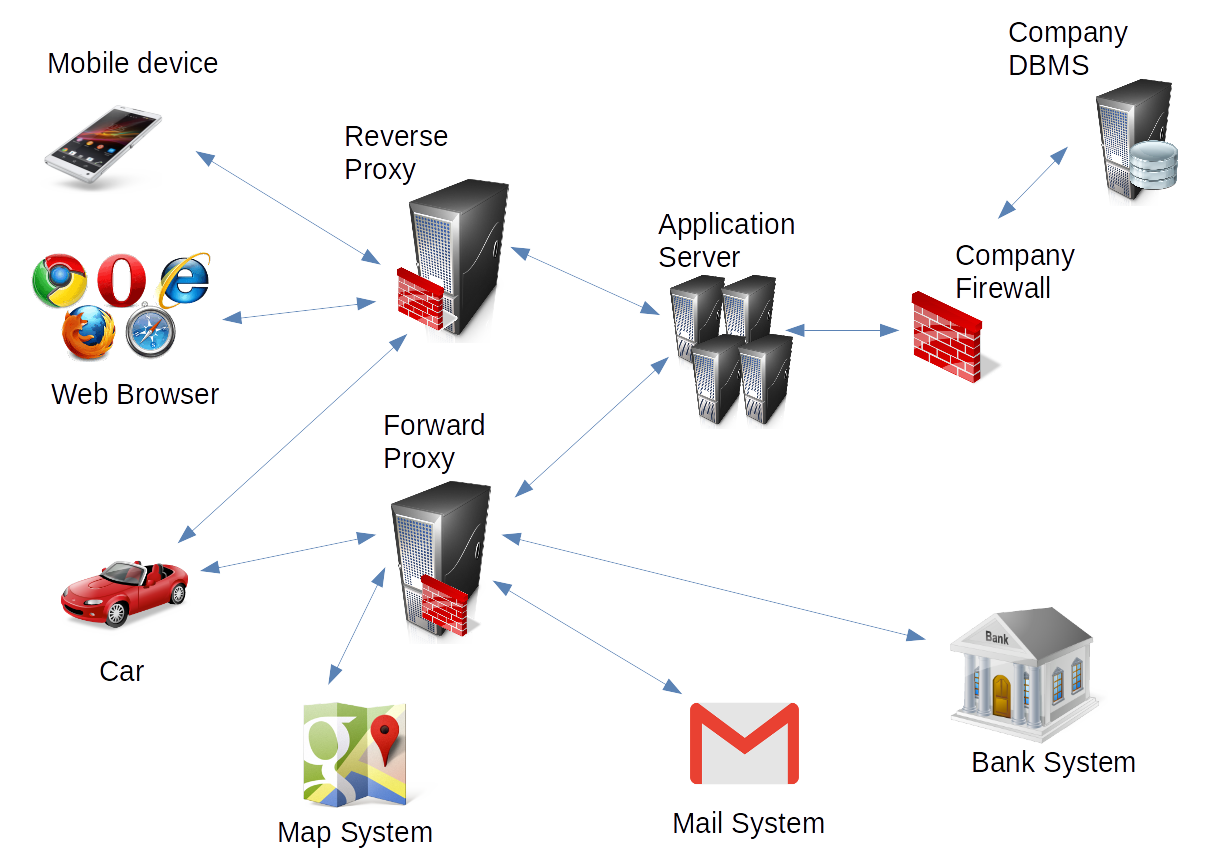
\includegraphics[width=\textwidth]{../Images/Overview}
	\caption{An overview of the System}
	\label{fig:overview}
\end{figure}


\subsection{Component View}
\begin{figure}[h]
	\centering
	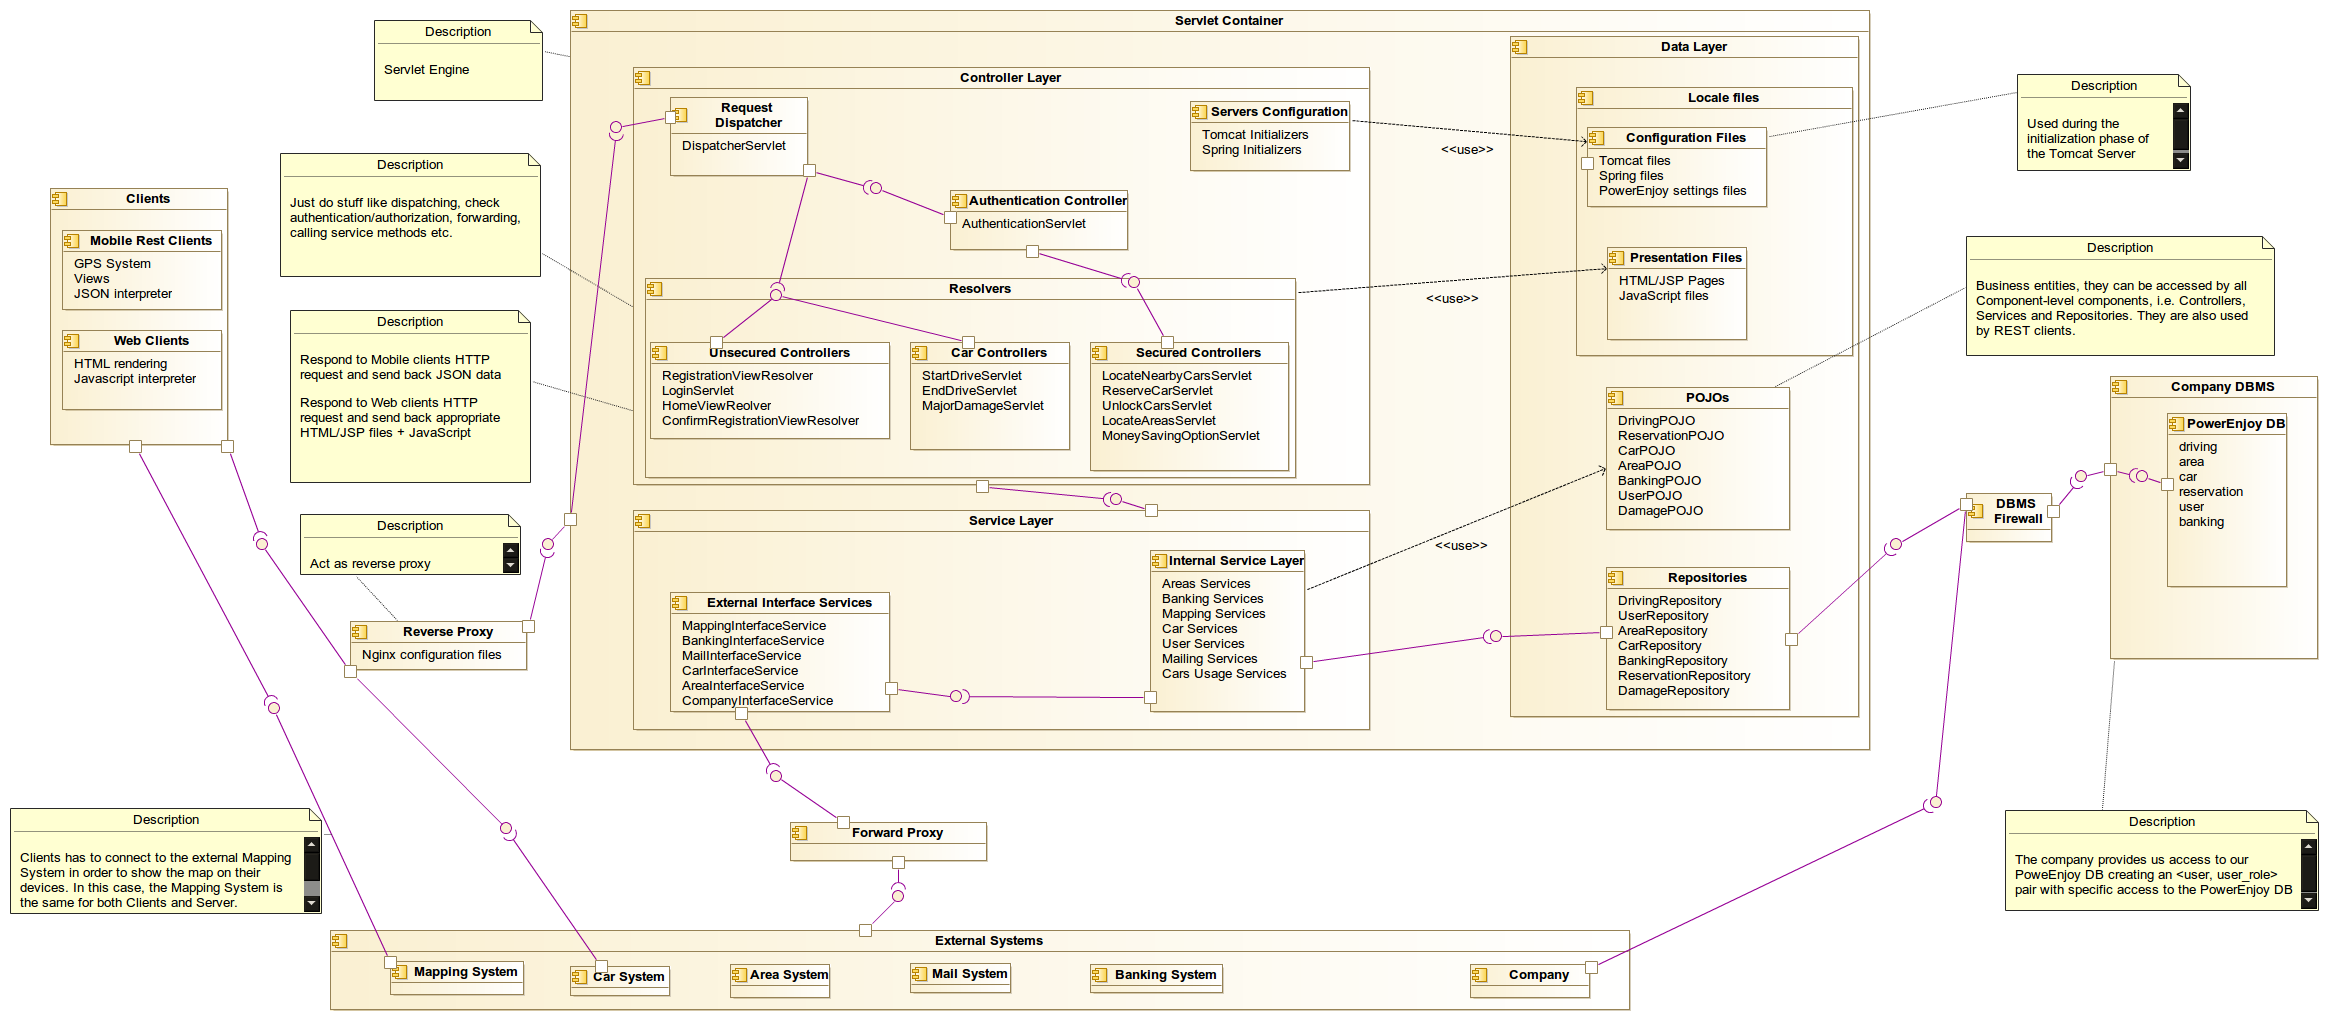
\includegraphics[width=\textwidth]{../Images/Component}
	\caption{Component Diagram}
	\label{fig:component}
\end{figure}
Image \ref{fig:component} shows the various System components and their relationship with each other. 

We can see three different kind of clients for our System:
\begin{itemize}
\item\textbf{Web Clients} represent the web browser that Users can use to access the System. The System returns simple HTML/JSP pages to them.
\item\textbf{Mobile Rest Clients} mainly represent all the clients that uses a RESTful approach to access the System functionalities. The main kind of Rest Clients are surely the user Devices on which the PowerEnjoy App is running, though it is surely possible to access the System functionalities through other kind of clients, provided them invokes the correct URLs. As we can see, it is required that the PowerEnjoy App has access to the GPS System of the Client in order to fullfil some of the requests and an external Map System used to show different kind of maps to the User.
\item\textbf{Car Systems} can access the System in order to send useful data of the Cars. This is due to the fact that, instead of continuously make the Server polling all the Cars for their data, we decided to install a board on each Car that sends data on specific, meaningful events.
\end{itemize}

The main part of the Component Diagram (and as a consequence of the entire System) is the Server, named as Servlet Container. In fact, in our approach, given the used technologies, the Server should be a Java Servlet Container (see also \ref{par:tomcat}).
Inside it, you can see the Spring Framework, which is the core component of the Server and that provides some interesting features to manage all the other components (see also \ref{Spring}).

Spring’s web module includes, among the others, two interesting beans that is worth mentioning:
\begin{itemize}
\item A \textit{DispatcherServlet}. Spring’s web MVC framework is, like many other web MVC frameworks, request-driven, designed around a central Servlet that dispatches requests to controllers and offers other functionality that facilitates the development of web applications. In practice, all the requests coming from clients are intercepted by the DispatcherServlet and redirected to the appropriate controllers: it is an expression of the "Front Controller" design pattern, a pattern that Spring Web MVC shares with many other leading web frameworks.
Note that we can achieve analogous results using the default JEE framework, but obviously Spring greatly simplifies our tasks.
\item Various \textit{Configuration classes} used to configure all the relevant aspects of the framework. Among them, for example, we have the \textit{WebApplicationInitializer}, that ensures the code-based configuration is detected and automatically used to initialize any Servlet 3 container.
\end{itemize}

\bigskip

The core logic of the System is encapsulated in the @Component, a name which is used to honour the Spring name. 
A @Component is a generic stereotype for any Spring-managed component. As such, all the @Component s are auto detectable by spring container and we don't need to define bean in configuration file because they will be automatically detected at runtime by Spring.

@Repository, @Service, and @Controller, on the other hand, are specializations of @Component for more specific use cases, namely the persistence layer, the service layer and the presentation layer respectively. Obviously, the use of the specialized stereotypes is encouraged, because on one hand they can provide further functionalities (such as the automatic translation of database exceptions for @Repository), and on the other they are useful to separate the layers of the application.

In addition to that, we use a specialized kind of @Controller, namely @RestController, to implement the RESTful pattern and responds to specific HTTP requests coming from RestClients and Devices.

We can also note the use of an authentication controller. Its role is to grant the access to specific controllers only to authenticated users, id est users already registered to the System and which has provided the correct access identifiers.

All the Controllers can/should use one or more services in order to correctly elaborate client requests.

\bigskip

For the @Service layer, we decided to separate the logic into two different components:
\begin{itemize}
\item The external service component are a simply interface between the System and external services. They are used to wrap invocations to external System methods into our methods, ensuring in this way that changes in the external System APIs can be managed only by the appropriate external service class, while at the same time not affecting the behaviour of any other class. They are invoked by the internal services to process transactions.
\item The internal service component are related to the core business logic of the System and are directly invoked by @Controllers or by other services to fullfil specific tasks. A specialized class of them is involved into elaborating specific tasks in background on specific events. 
\end{itemize}

One thing is worth noting at this point: the Car System acts both as a Client and as a Server for our System. Indeed, as previously said, a Car can send data to the System at the occurrence of specific events. On the other hand, the System can query the Car status at any point for specific reasons. It is this the reason for which we must have a Car Interface Service.

\bigskip
The goal of the Spring @Repository is to significantly reduce the amount of boilerplate code required to implement data access layers for various persistence stores. In other words, it is used to provide a single way to access different type of data storage implementations. Indeed, you can use specific naming conventions for the methods of the repository classes and the framework automatically translates them into queries specific for the underlying data storage.

The Repository pattern is in general slightly different from the DAO pattern, because it can manage aggregate data more than single data. However, in Spring the distinction between the two patterns is not so clear.
In our approach, we have repository classes for the most relevant entities of our database, while other entities can be accessed indirectly.

\bigskip
Last but not least, in our Server we have to provide the JPA @Entity annotation on those classes that are directly mapped into the database. In other words, the @Entity annotation is used to define classes whose instances can be stored in a database.

\subsection{Class View}
The following diagrams show the Class Diagrams for various parts of the System.
We then have a diagram showing the relationships between the POJOs, the Objects that make up the Persistence layer, and finally one for the tasks that are constantly running on the Server.

\begin{figure}[h]
	\centering
	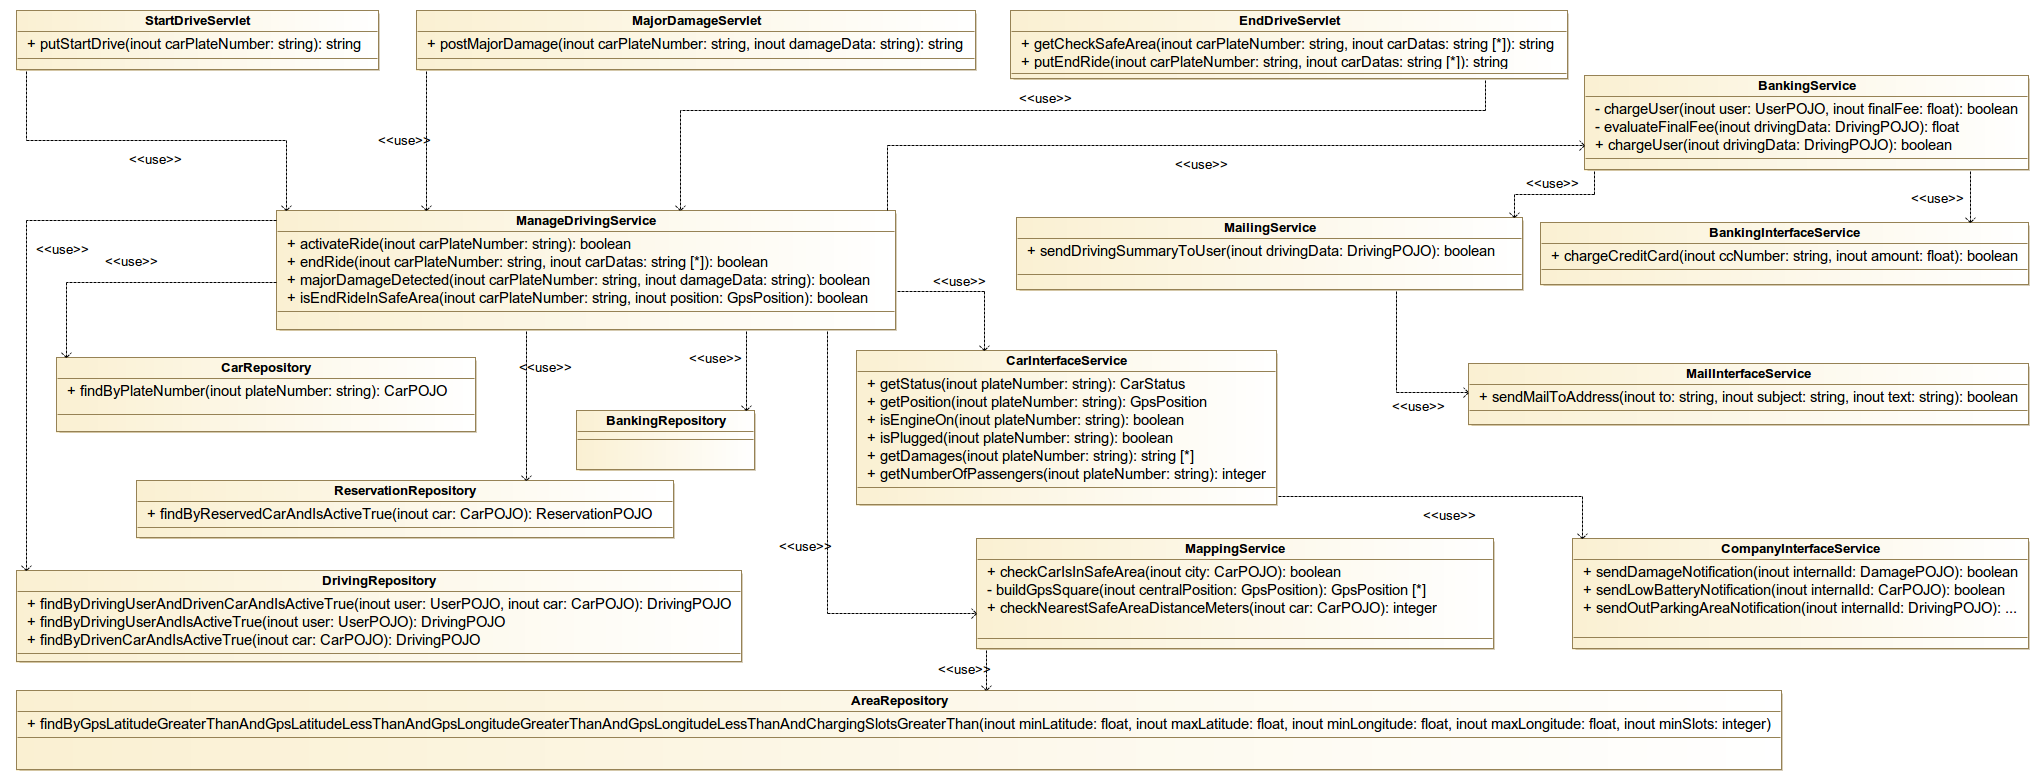
\includegraphics[width=\textwidth]{../Images/CarClient_Class}
	\caption{Class Diagram for the Car Client}
\end{figure}

\begin{figure}[h]
	\centering
	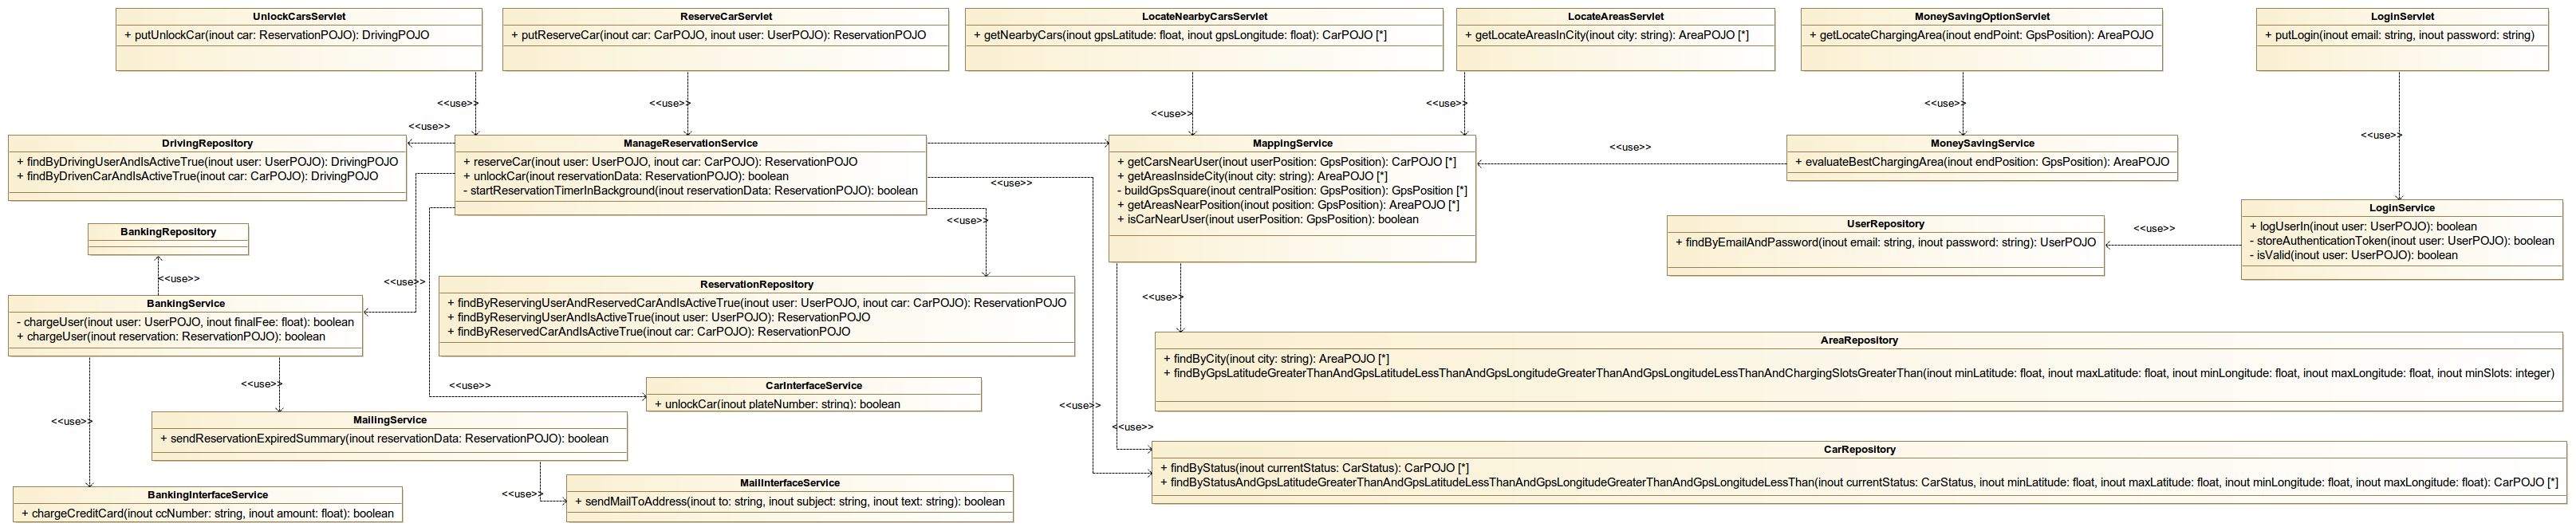
\includegraphics[width=\textwidth]{../Images/MobileClient_Class}
	\caption{Class Diagram for the Mobile Client}
\end{figure}

\begin{figure}[h]
	\centering
	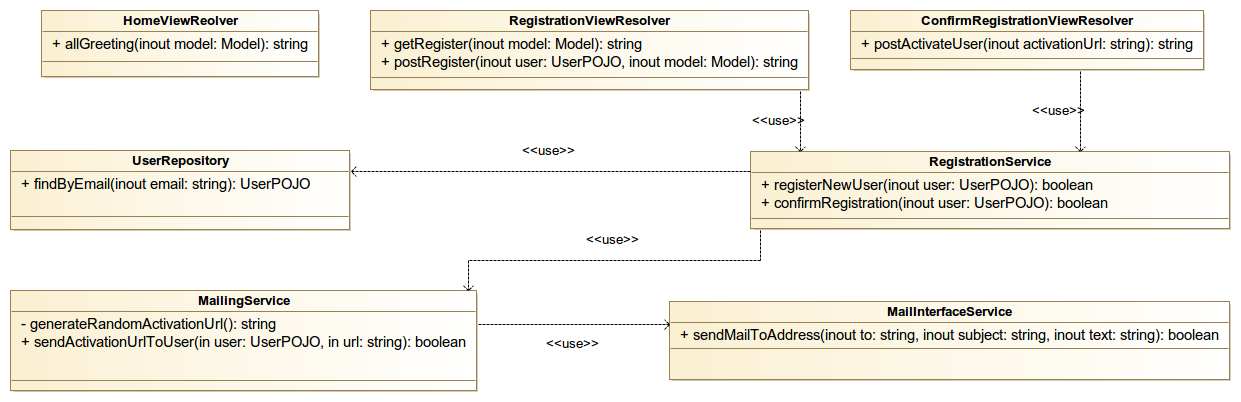
\includegraphics[width=\textwidth]{../Images/WebClient_Class}
	\caption{Class Diagram for the Web Client}
\end{figure}

\begin{figure}[h]
	\centering
	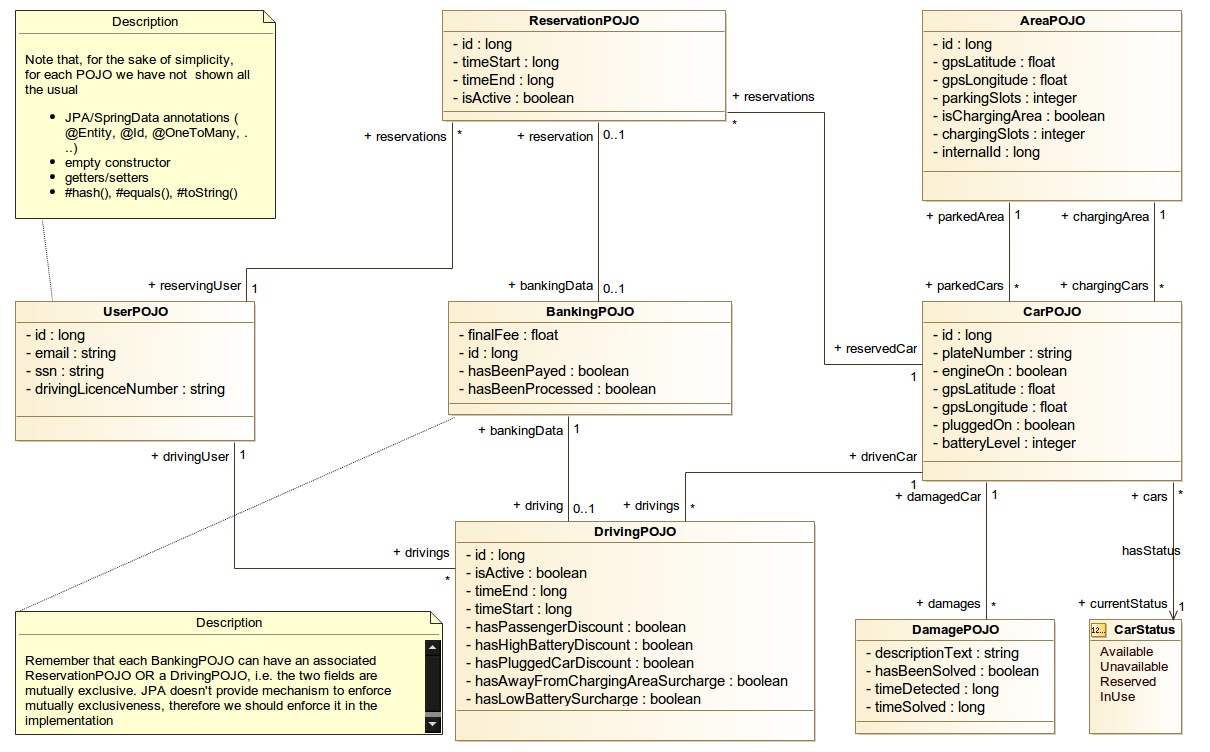
\includegraphics[width=\textwidth]{../Images/POJOs}
	\caption{POJO Objects}
\end{figure}

\begin{figure}[h]
	\centering
	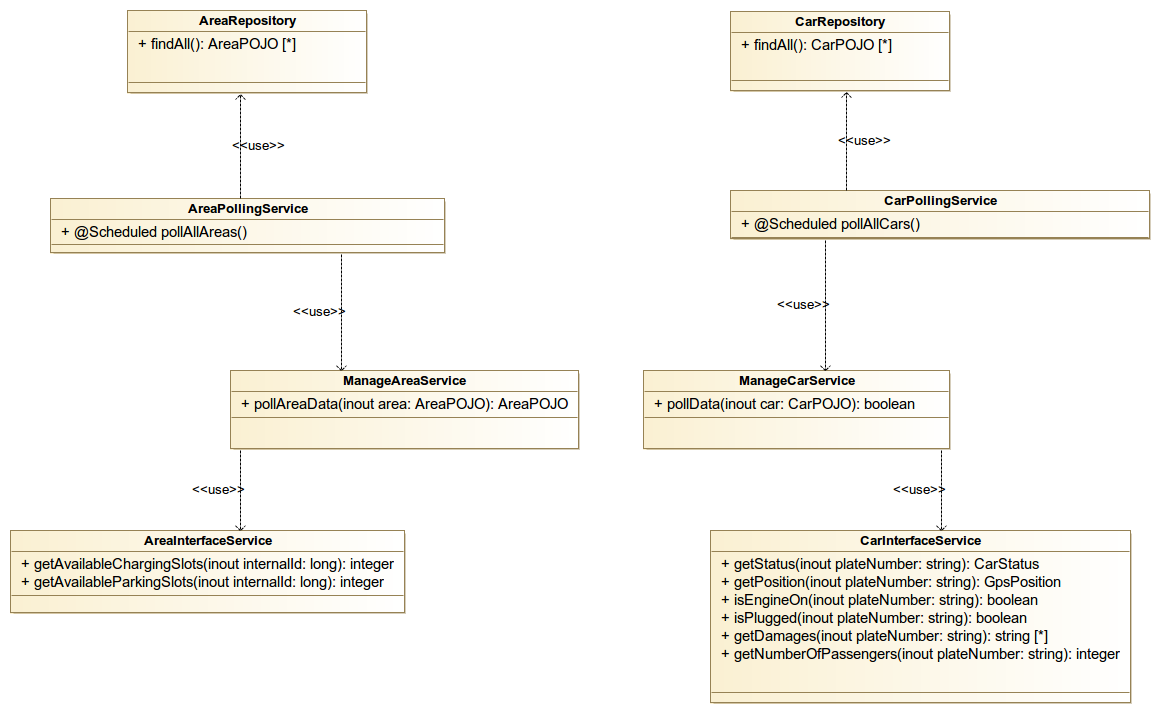
\includegraphics[width=\textwidth]{../Images/BackgroundTasks}
	\caption{Background Tasks}
\end{figure}
\clearpage

\subsection{Communication View}
The following diagrams are used to show the HTTP requests that Clients use to contact the server, along with the most relevant server responses.

\begin{figure}[h]
	\centering
	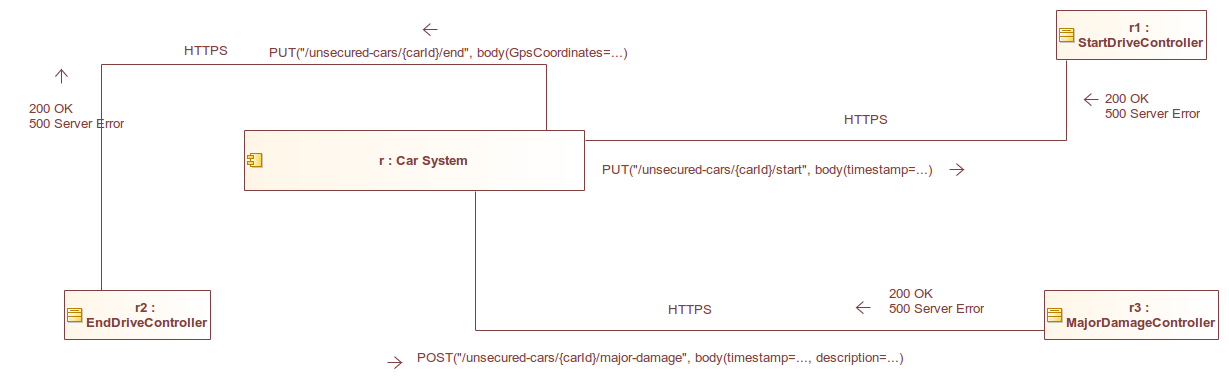
\includegraphics[width=\textwidth]{../Images/CarClient_Communication}
	\caption{Communication Diagram for Car Client}
\end{figure}

\begin{figure}[h]
	\centering
	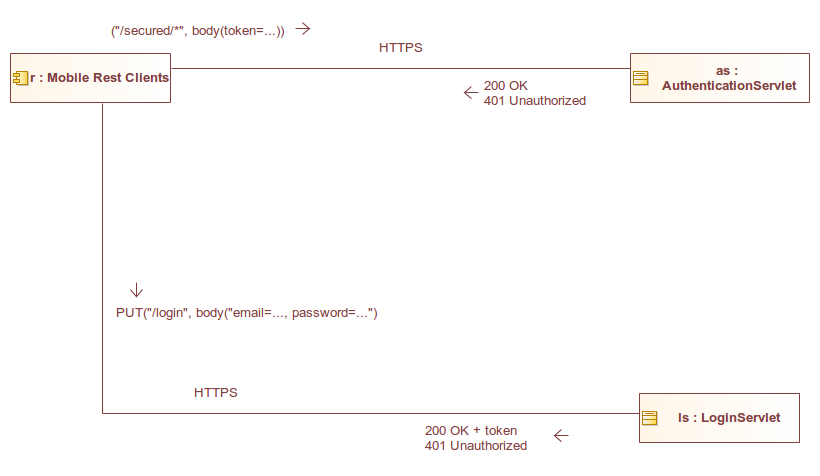
\includegraphics[width=\textwidth]{../Images/MobileAuth_Communication}
	\caption{Communication Diagram for Authenticator}
\end{figure}

\begin{figure}[h]
	\centering
	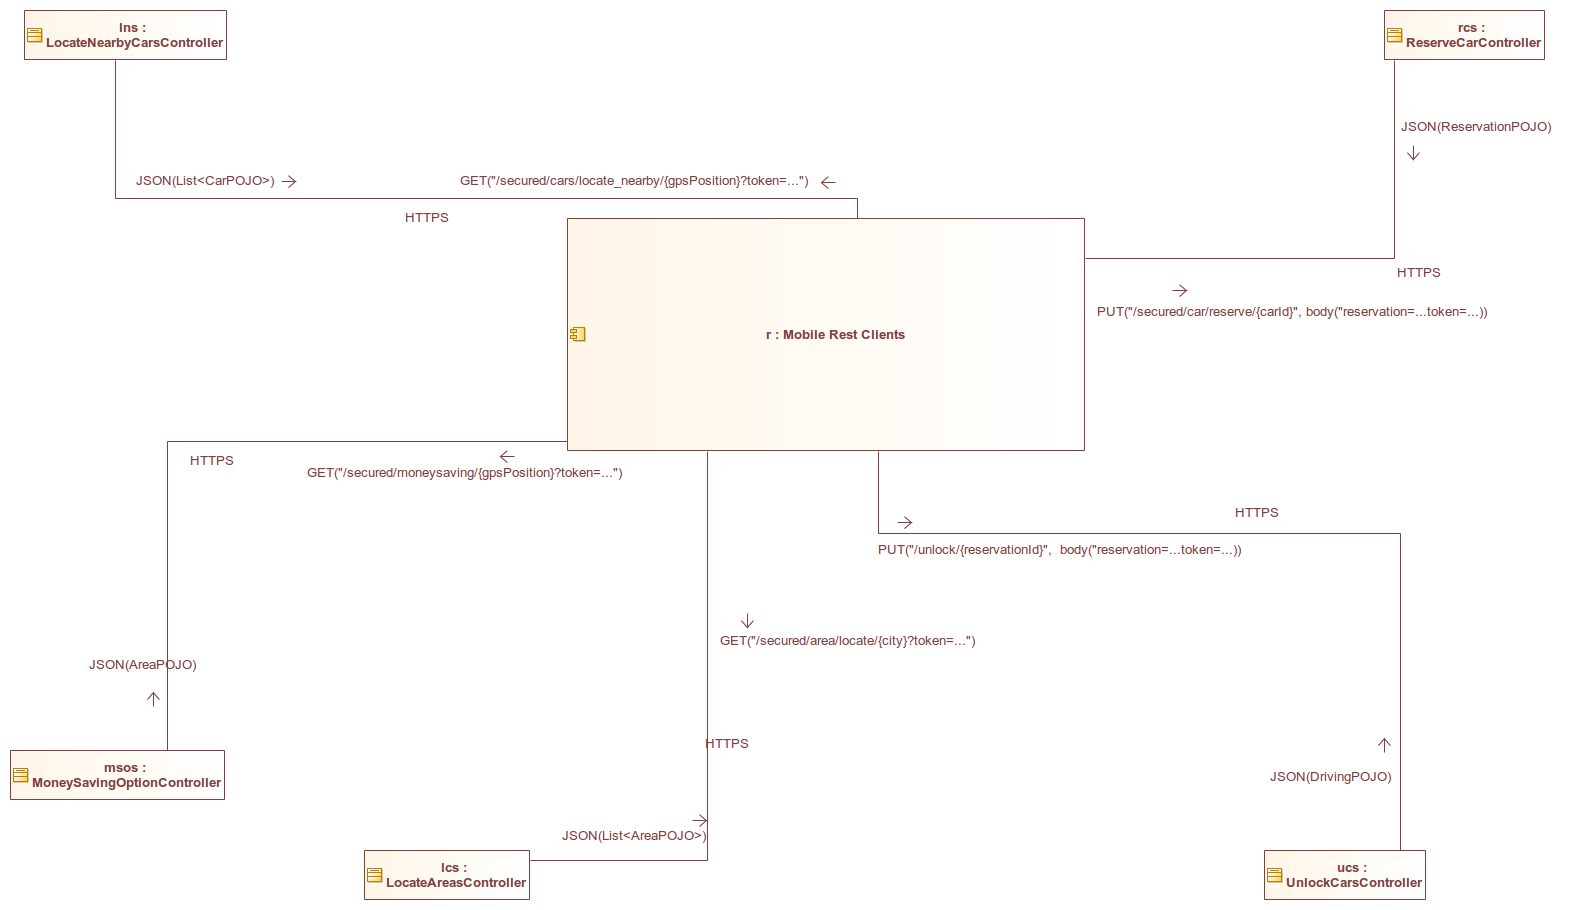
\includegraphics[width=\textwidth]{../Images/MobileClient_SecuredCommunication}
	\caption{Communication Diagram for Mobile Client Secure}
\end{figure}

\FloatBarrier

\begin{figure}[h]
	\centering
	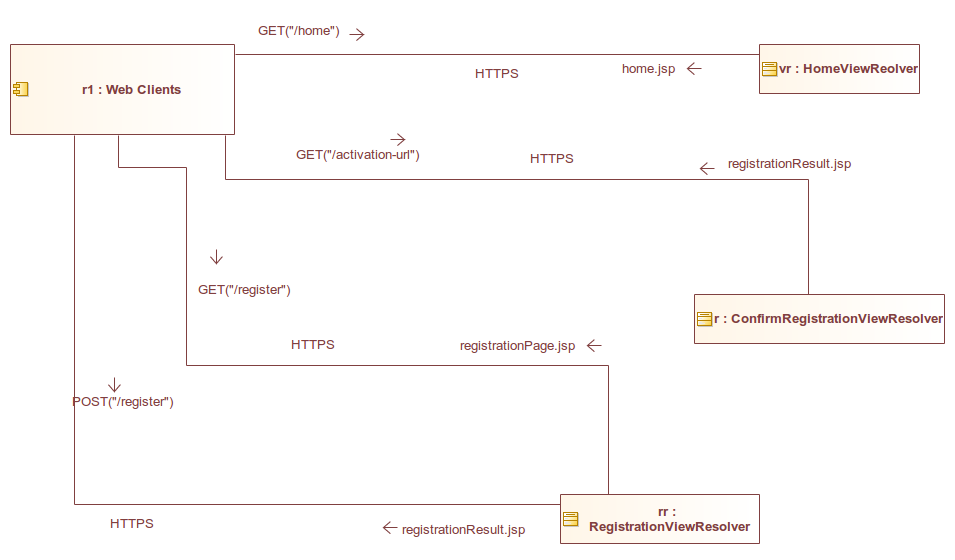
\includegraphics[width=\textwidth]{../Images/WebClient_Communication}
	\caption{Communication Diagram for Web Client}
\end{figure}

Is it interesting to note that while to requests from Web Clients the Server responds with HTML/JSP files, for the Mobile Clients and Car Clients it returns JSON data which must be correctly processed by the clients.

We can also that the secured connection between Mobile Clients and the server is ensured by the use of a token, which is generated by the Server on a successful login and then sent back to the client. On subsequent access, the clients should send this token in order to access secured resources.

\subsection{Deployment View}
The following diagram shows the deployment view of the whole System. The server specifications are described in \ref{server}.
\begin{figure}[h]
	\centering
	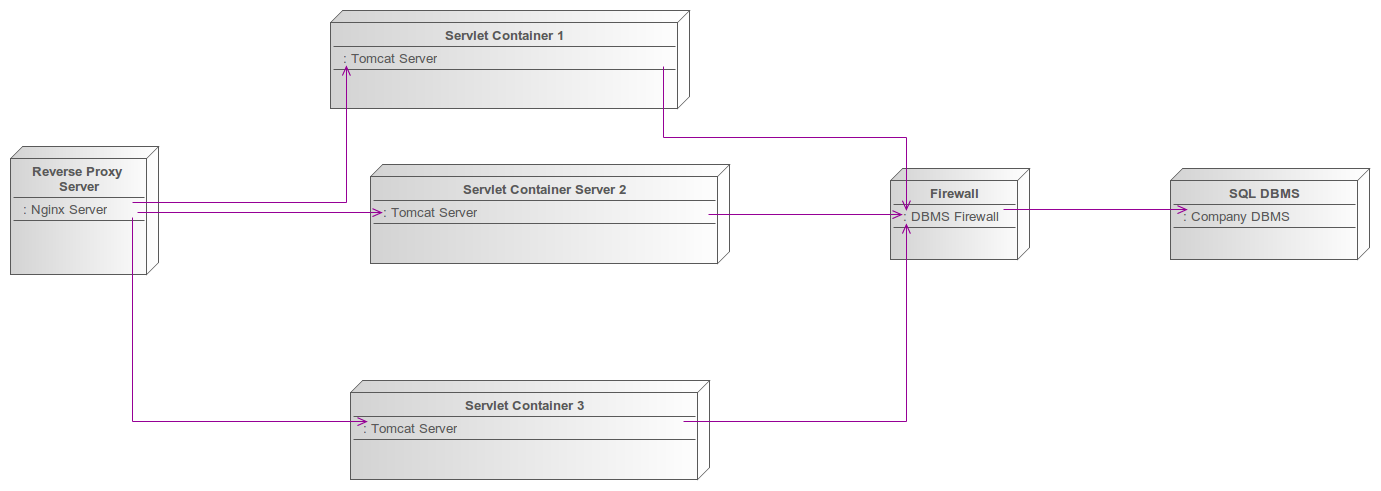
\includegraphics[width=\textwidth]{../Images/Deployment}
	\caption{Deployment Diagram}
\end{figure}

As per the overview diagram in figure \ref{fig:overview}, we introduced also some security layers between the various part of our System.

The Reverse Proxy is a type of proxy server that retrieves resources on behalf of a client from one or more servers. These resources are then returned to the client as if they originated from the proxy server itself. Among the others, a reverse proxy is useful for the following reasons:
\begin{itemize}
\item Application firewall features can protect against common web-based attacks, such as DoS or DDoS. Without a reverse proxy, removing malware or initiating takedowns, for example, can become difficult.
\item In the case of secure websites, a web server may not perform SSL encryption itself, but instead offloads the task to a reverse proxy that may be equipped with SSL acceleration hardware.
\item A reverse proxy can distribute the load from incoming requests to several servers, with each server serving its own application area. In the case of reverse proxying in the neighborhood of web servers, the reverse proxy may have to rewrite the URL in each incoming request in order to match the relevant internal location of the requested resource.
\item Reverse proxies can operate wherever multiple web-servers must be accessible via a single public IP address. The web servers listen on different ports in the same machine, with the same local IP address or, possibly, on different machines and different local IP addresses altogether. The reverse proxy analyzes each incoming request and delivers it to the right server within the local area network.
\end{itemize}

We choose to deploy the reverse proxy on a Linux machine, inside which we used the Nginx server to easily configure all the relevant aspects.

\bigskip
The Server is instead deployed on two different Linux machines which runs the Tomcat server, an open source Java Servlet container.
Whenever the Server must invoke the methods of external systems, its requests are handled by the forward proxy. Basically, it acts as an intermediary for requests from clients (in this case our Server) seeking resources from other servers (the external systems). Among other well-known capabilities provided by a forward proxy, we must note the added security layer introduced by its use. Indeed, a proxy can keep the internal network structure of the company secret by using network address translation. This makes requests from machines and users on the local network anonymous. 
We choose to use Tinyproxy, a fast and small open source implementation of a proxy server, which will run on a single Linux machine.

\bigskip
The access to the Database is also mediated by a firewall, whose capabilities are well-known and beyond the scope of this document.

\clearpage

\subsection{Runtime View}
\subsubsection{Registration}
\begin{figure}[h]
	\centering
	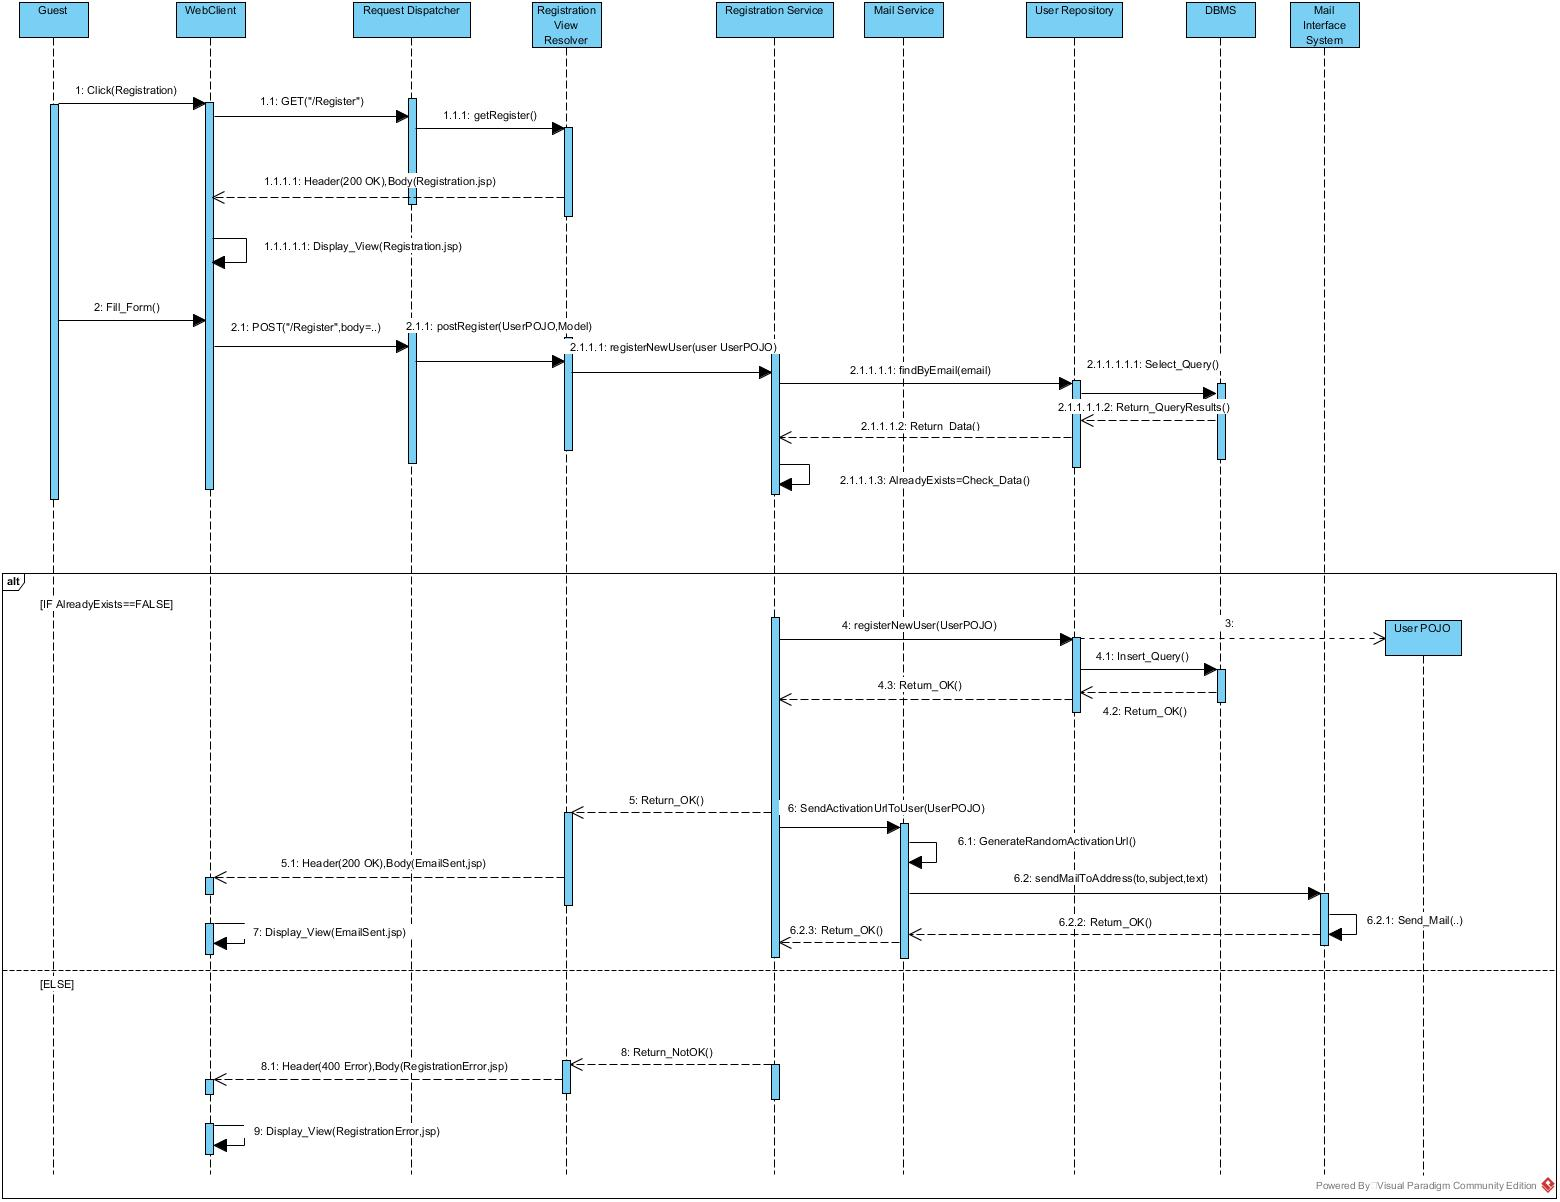
\includegraphics[width=\textwidth]{../Images/Sequence_Final/Registration}
	\caption{Registration}
\end{figure}

\begin{figure}[h]
	\centering
	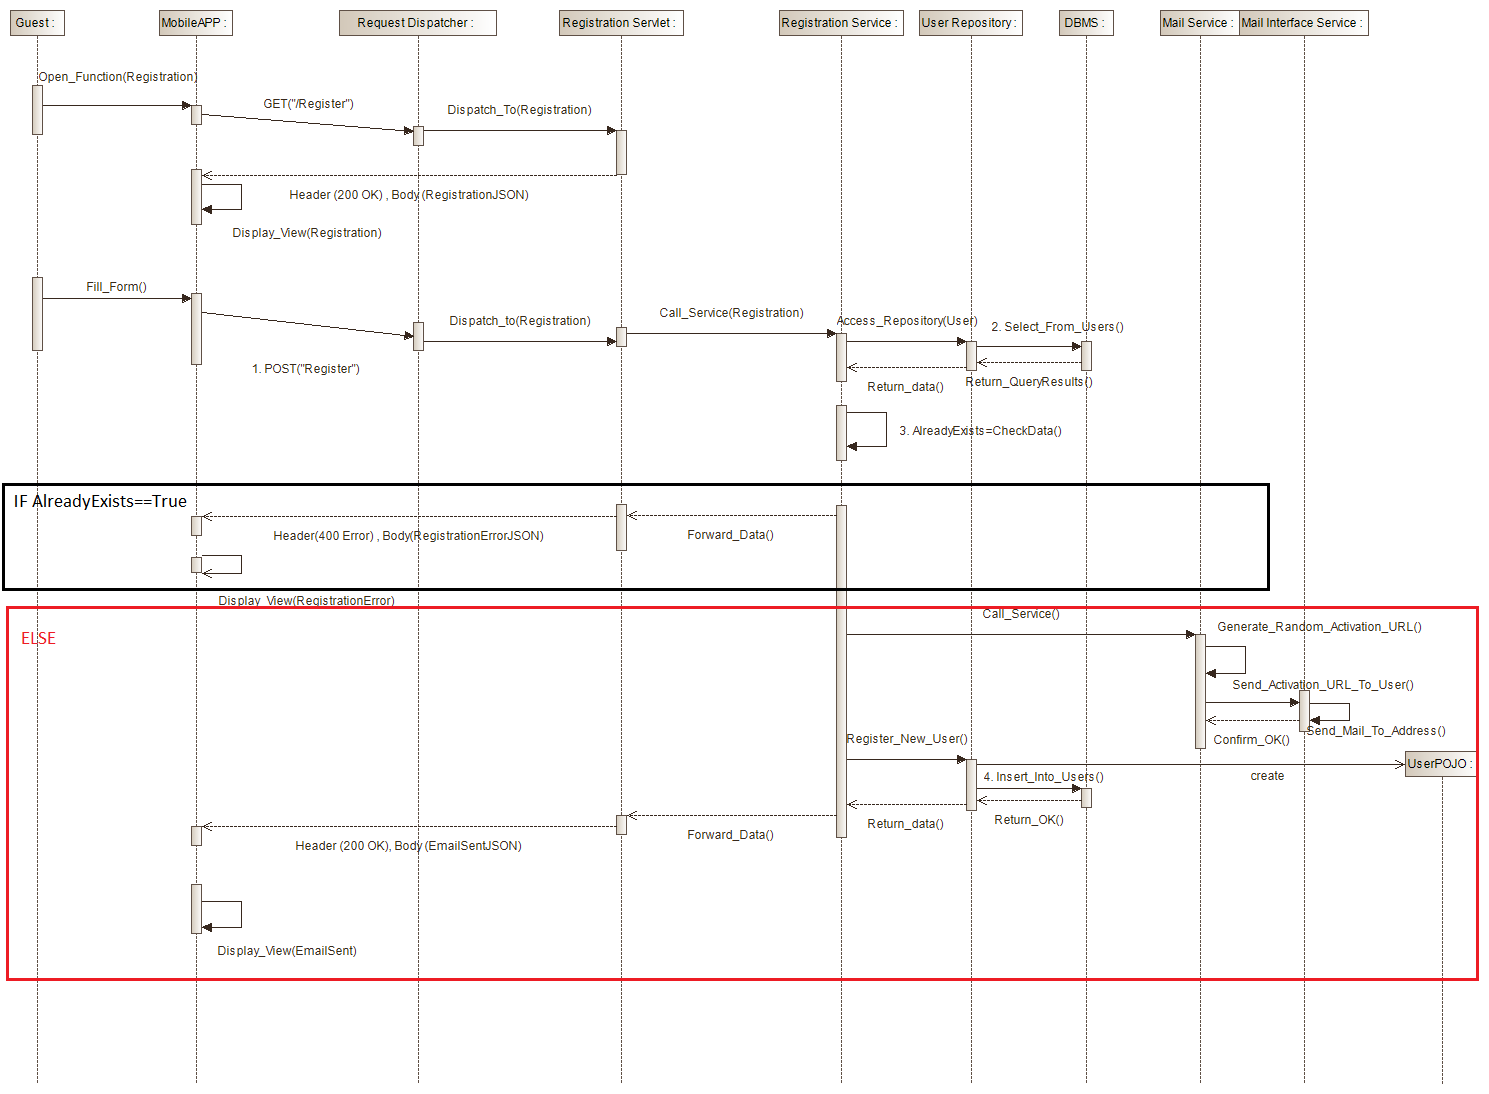
\includegraphics[width=\textwidth]{../Images/Sequence_Final/Registration_Mobile}
	\caption{Registration from Mobile}
\end{figure}

The Visitor wants to register to this platform to have access to the PowerEnjoy services.
We decided to give the option to register both via mobileapp and via browser. 
In the MobileApp case the data are sent through JSON while in the browser we return data through JSP.
\begin{enumerate}
	\item[1.] The Visitor fills the registration form writing their DrivingLicenseNumber, NumberIDCard , email, password and others non-mandatory data (e.g. date of birth). This data will be sent via the POST HTTP method.
	\item[2-3.] The System performs a SQL Query to the Database and checks if there are already other accounts with the same email, DrivingLicenseNumber or NumberIDCard. In this way we are sure the Visitor has one account only. If there is another account with those credentials we show an error message to the Visitor, inviting them to login.
	\item[4.] If nothing went wrong we insert a new tuple with the Visitor's Data into the Table USERS. 
\end{enumerate}
\clearpage
\subsubsection{Confirm Mail}
\begin{figure}[h]
	\centering
	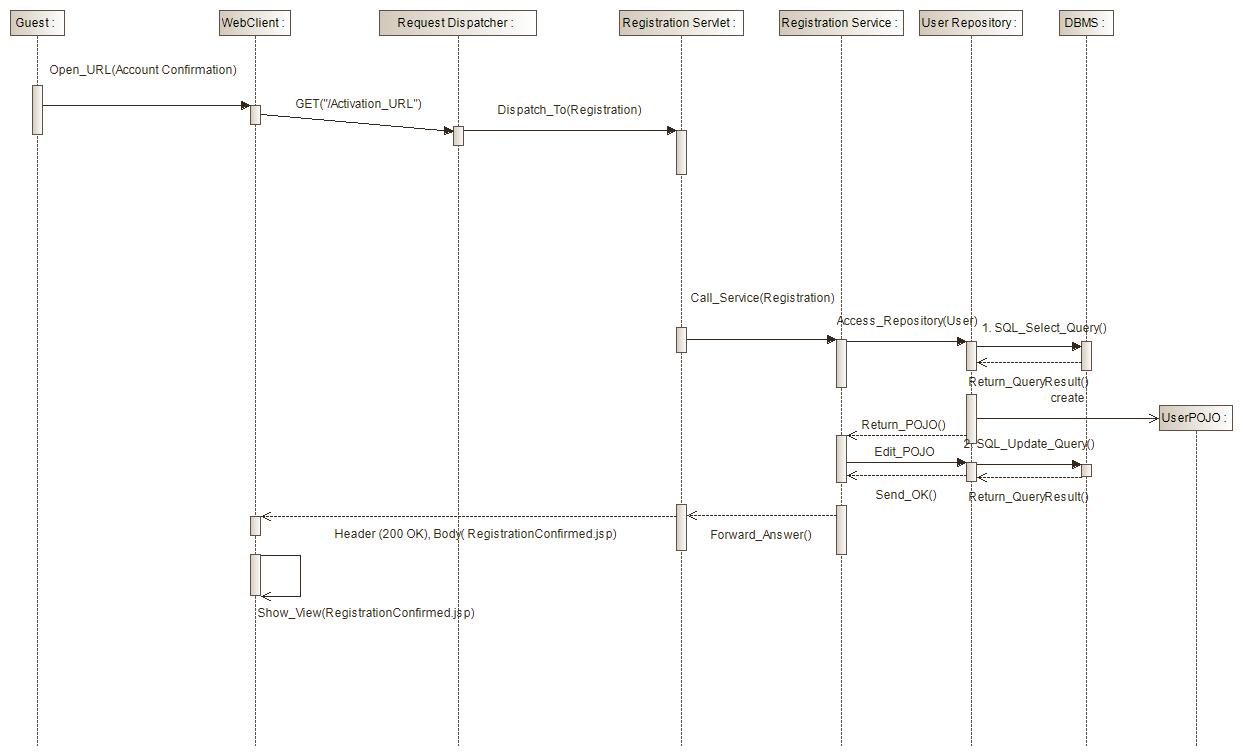
\includegraphics[width=\textwidth]{../Images/Sequence_Final/Confirm_Email}
	\caption{Email Confirmation}
\end{figure}

The User will open the URL received in their mail to confirm his account. This action can only be performed via a Web Browser.
\begin{enumerate}
	\item[1.] The DataBase checks the existence of the tuple of the corresponding User from the Table USERS.
	\item[2.] We update the field concerning the confirmation of the account in the tuple of the corresponding User from the Table USERS.
\end{enumerate}
\clearpage
\subsubsection{Login}
\begin{figure}[h]
	\centering
	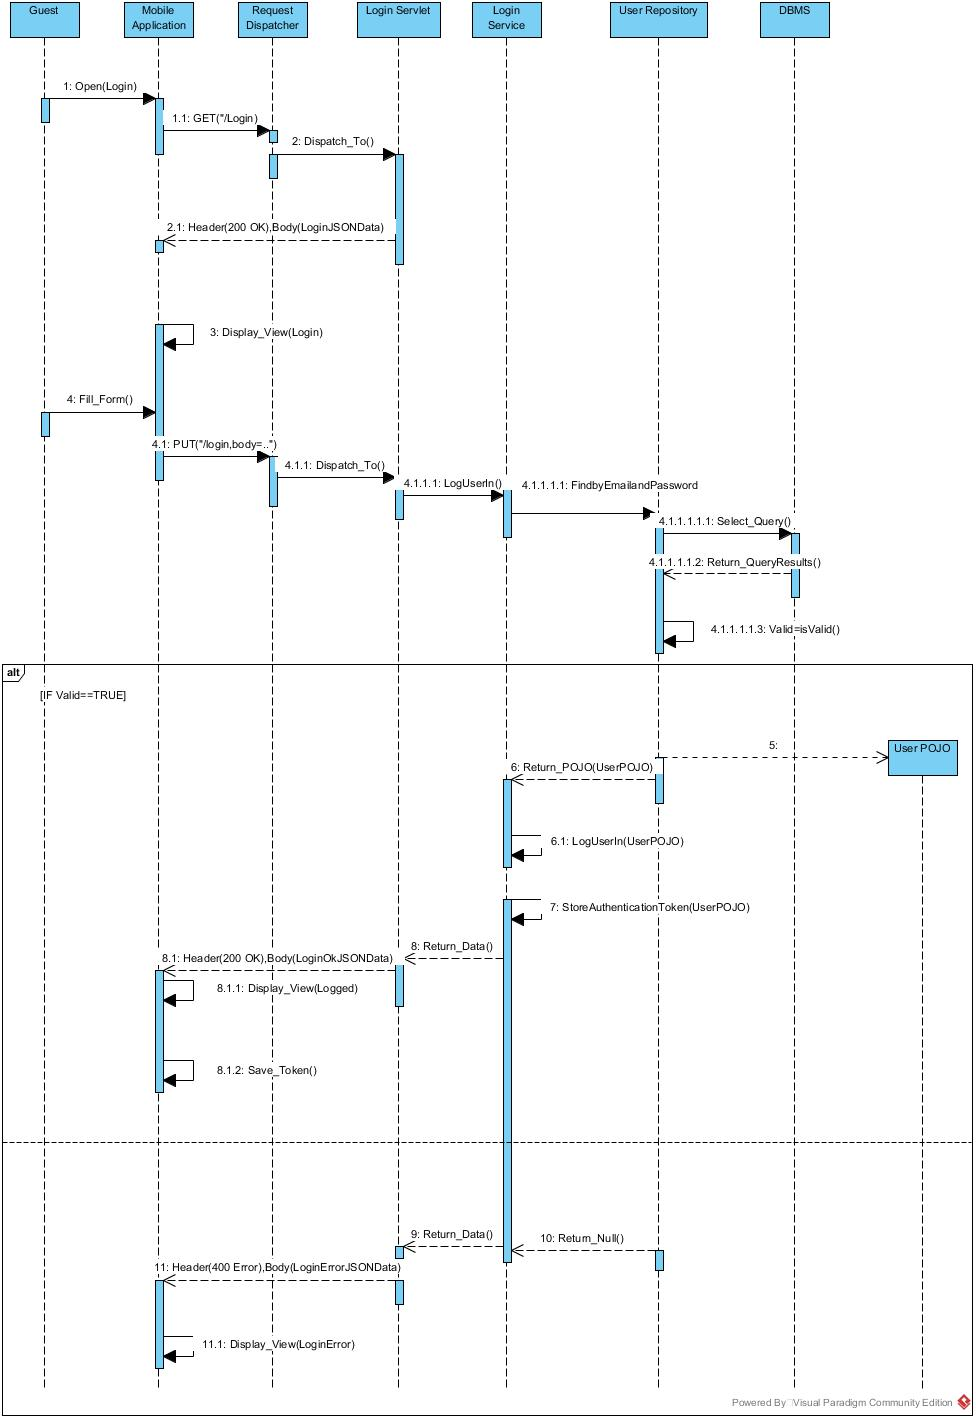
\includegraphics[width=\textwidth]{../Images/Sequence_Final/Login}
	\caption{Login}
\end{figure}

The User can perform this action via mobileAPP only.Moreover this action is required for all the incoming actions.
\begin{enumerate}
	\item[1.] The User inserts his credentials (email, password) to log in the System.
	\item[2.] We perform a SQL query to check if there exists a tuple with the user provided data (email and password). We update the field concerning the confirmation of the account in the tuple of the corresponding User from the Table USERS.
\end{enumerate}
\clearpage
\subsubsection{Show Areas}
\begin{figure}[h]
	\centering
	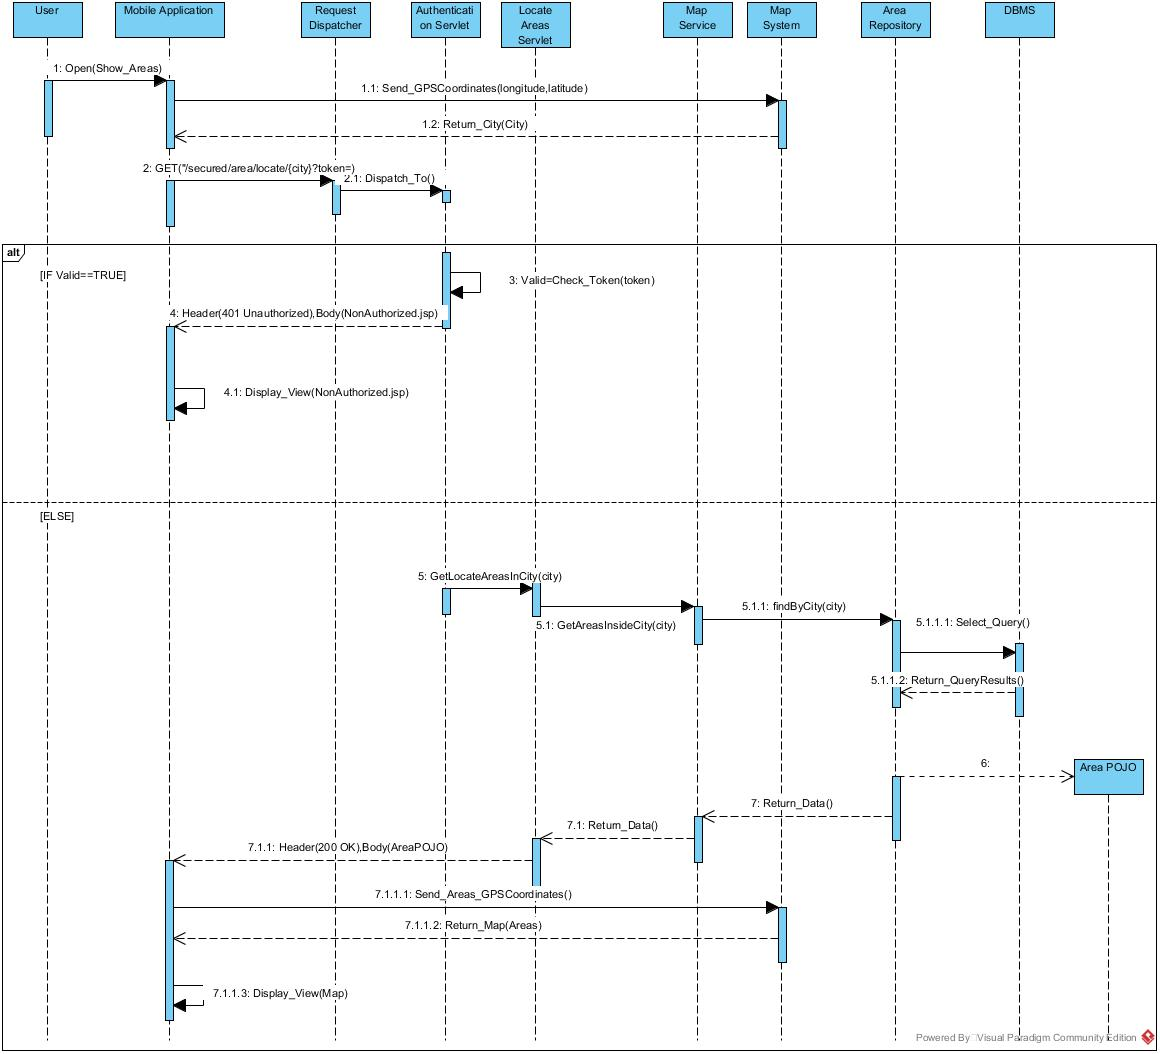
\includegraphics[width=\textwidth]{../Images/Sequence_Final/Show_Areas}
	\caption{Show Areas}
\end{figure}
The User can perform this action only via mobileAPP.
\begin{enumerate}
	\item[1.] GET(``/secured/area/locate/{city}?token=…'')
	\item[2.] We perform a SQL query to select the Areas that have a value of 'city' corresponding to the received Position.
\end{enumerate}
\clearpage
\subsubsection{Locate Cars}
\begin{figure}[h]
	\centering
	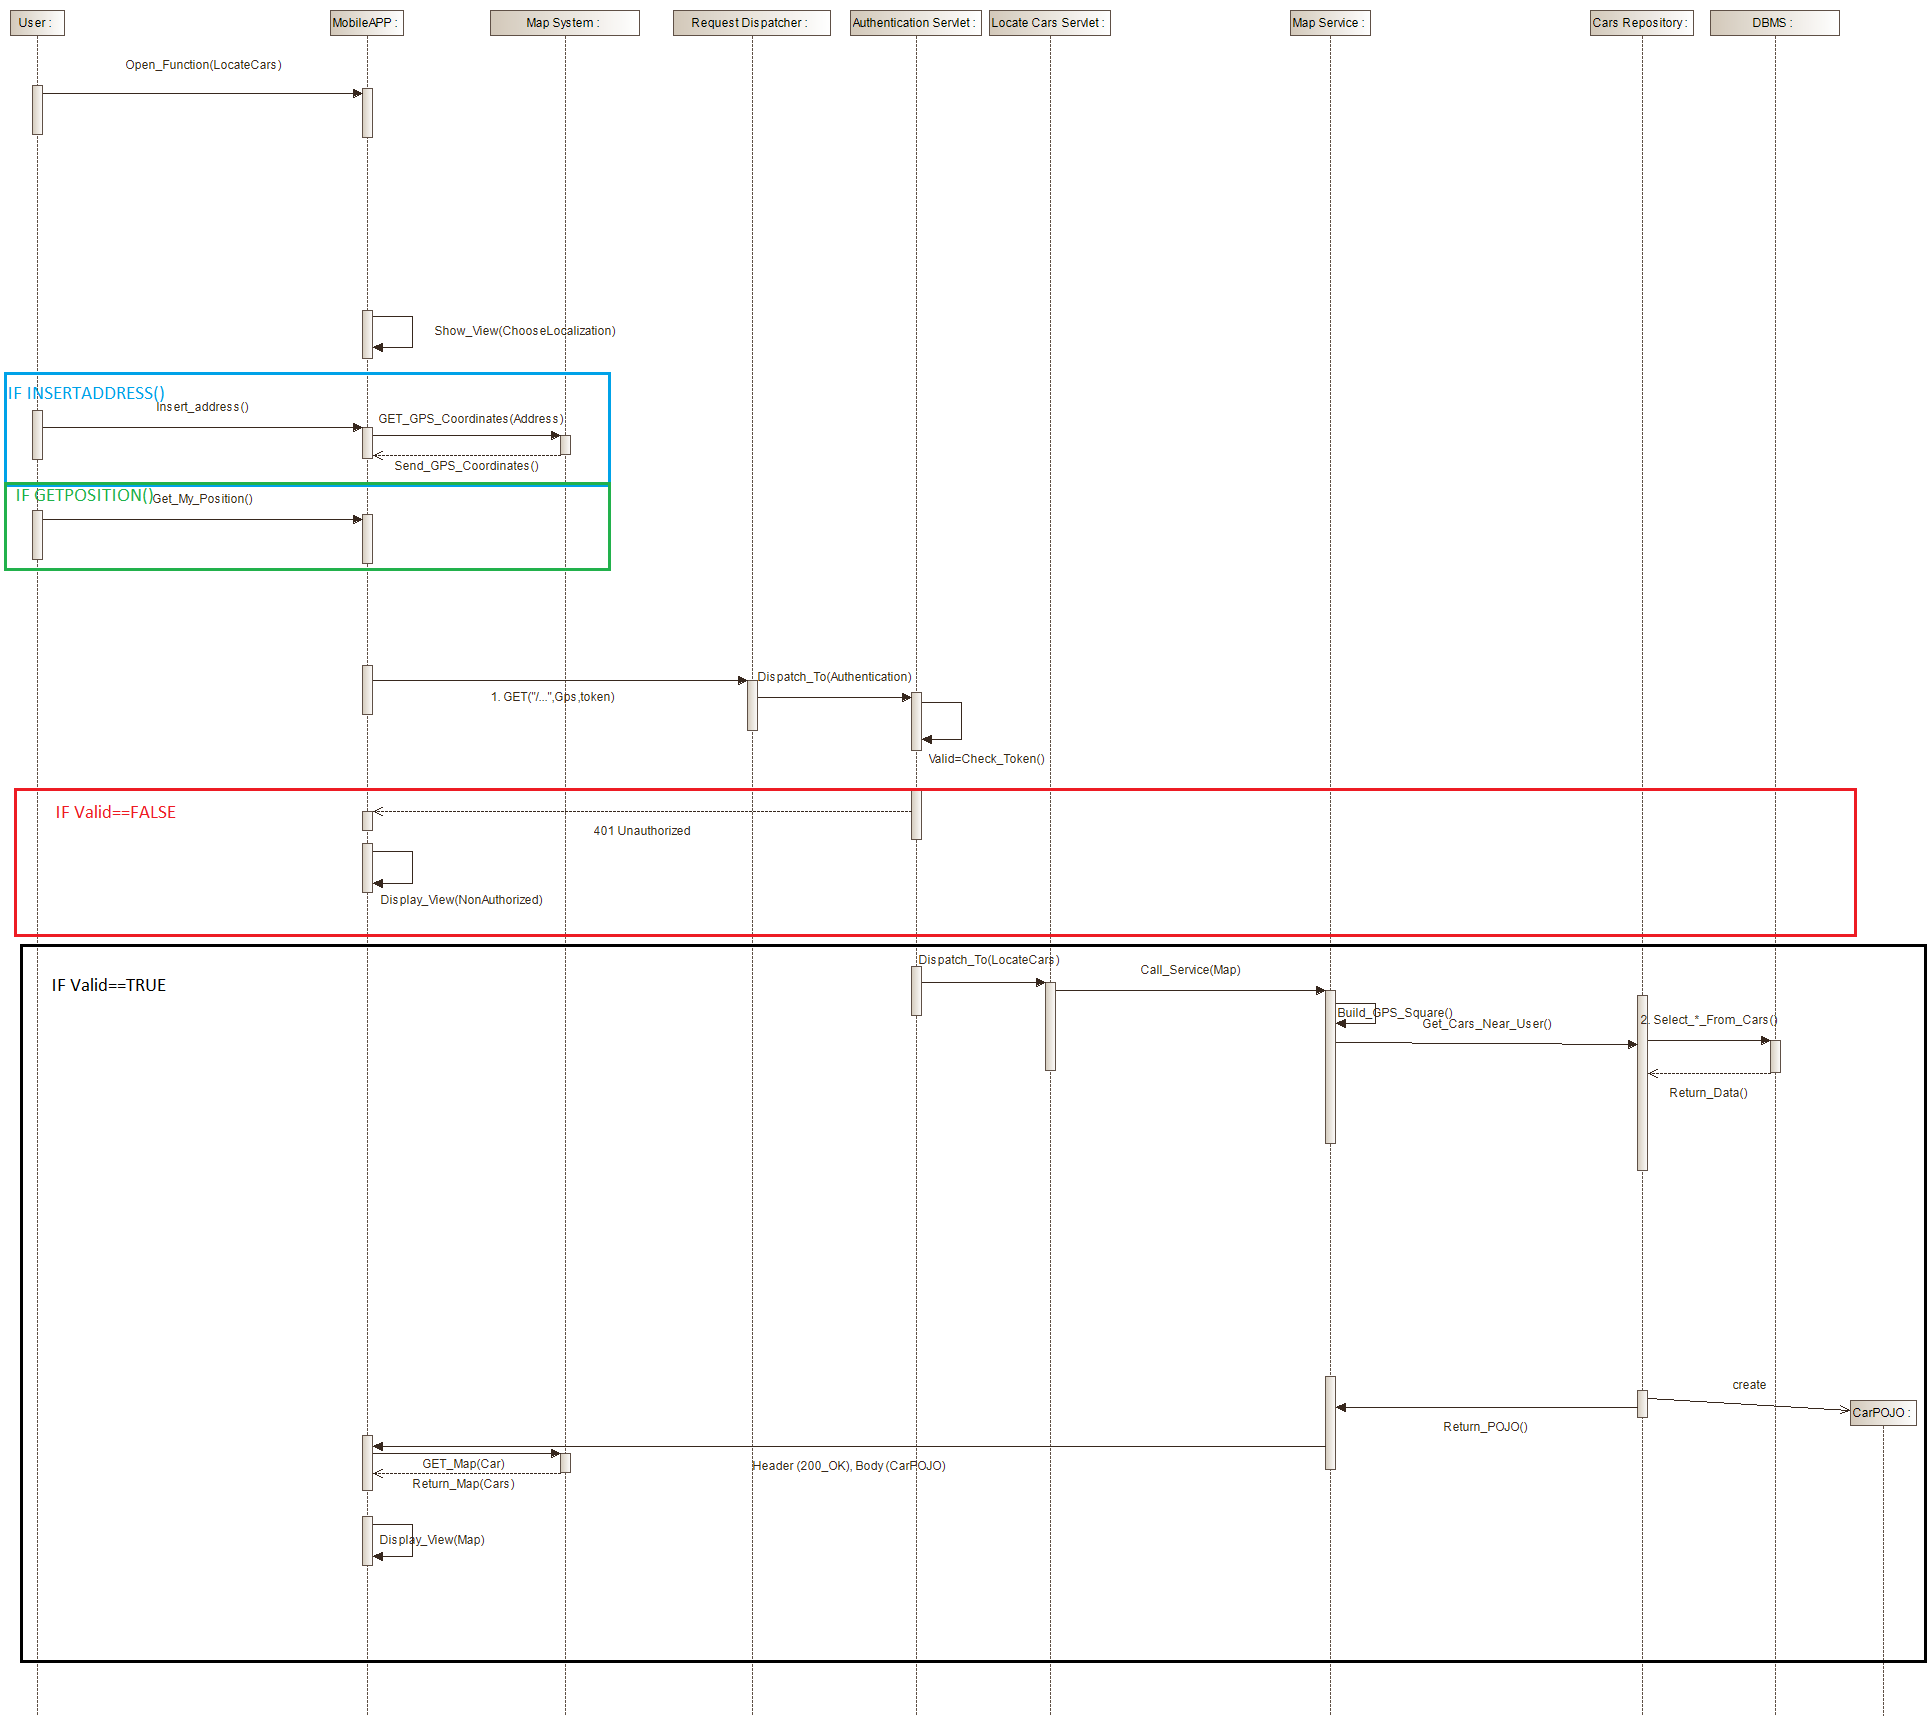
\includegraphics[width=\textwidth]{../Images/Sequence_Final/Locate_Cars}
	\caption{Locate Cars}
\end{figure}
The User can perform this action only via mobileAPP.
\begin{enumerate}
	\item[1.] GET(``/secured/cars/locate\_nearby/{gpsPosition}?token=…'')
	\item[2.] We perform a SQL query to select the Cars and select those which have GPS coordinates within the required bounds.
\end{enumerate}
\clearpage
\subsubsection{Reserve Car}
\begin{figure}[h]
	\centering
	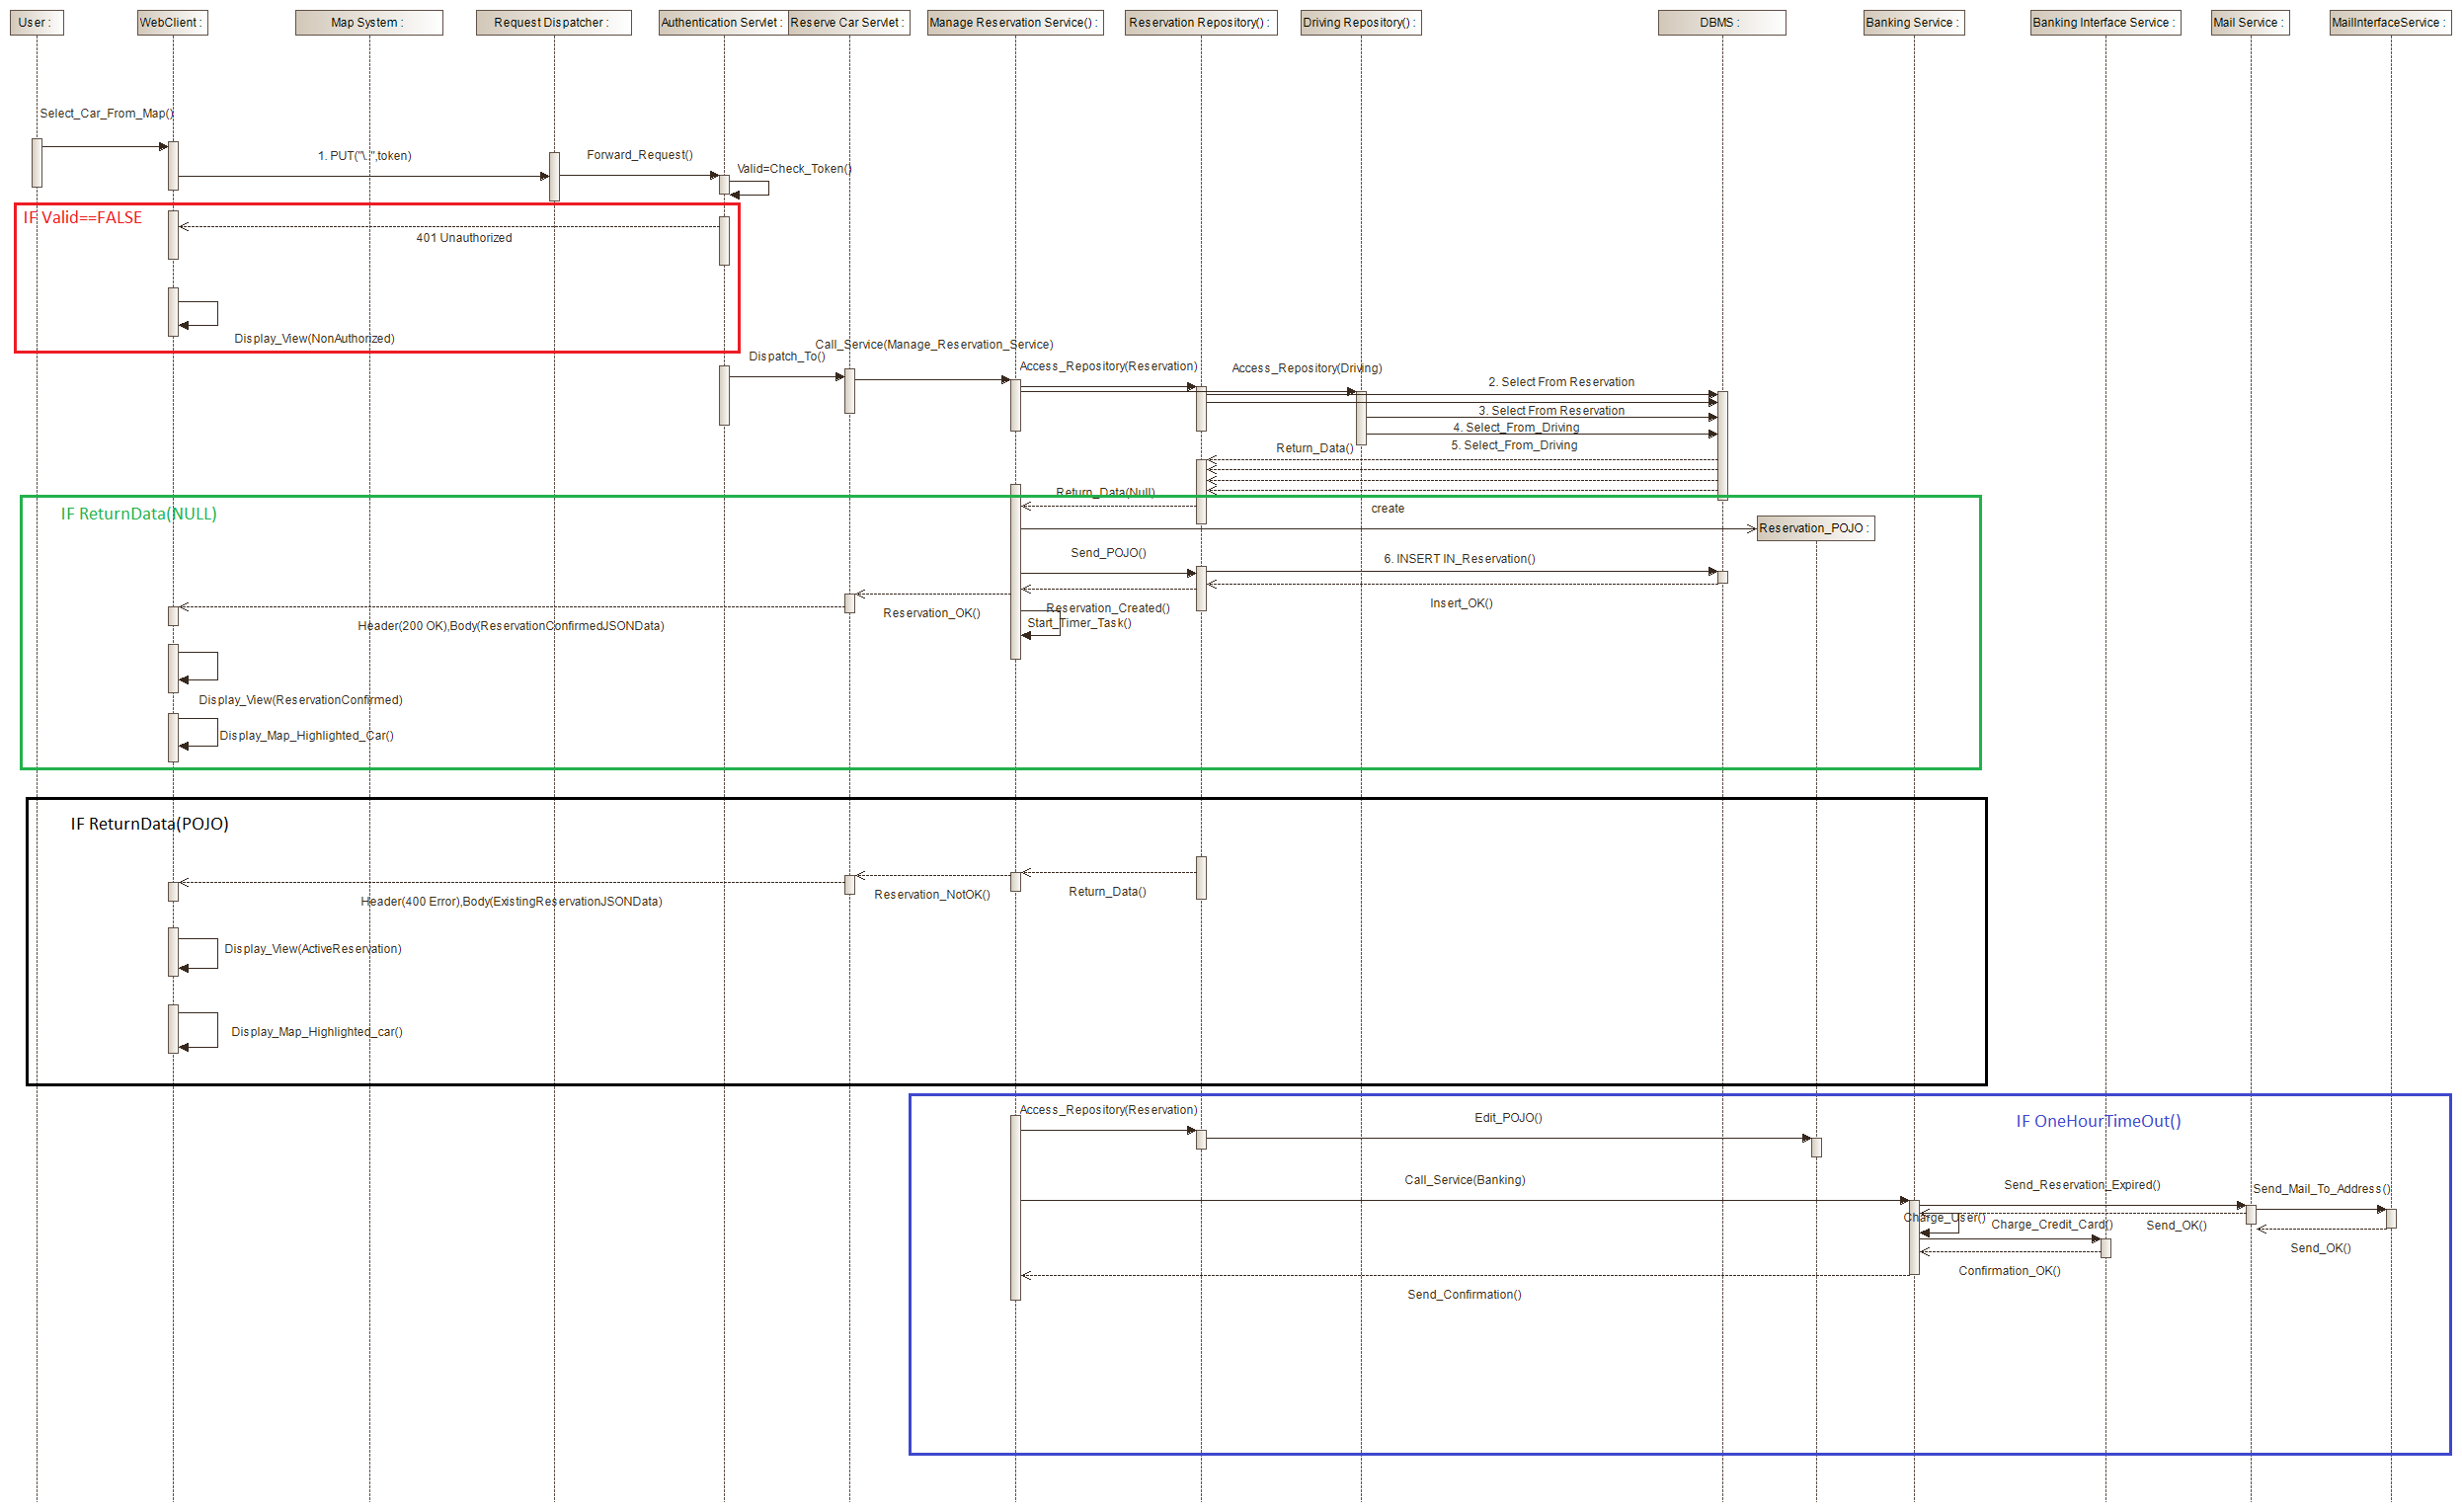
\includegraphics[width=\textwidth]{../Images/Sequence_Final/Reserve_Car}
	\caption{Reserve Car}
\end{figure}
\begin{enumerate}
	\item[1.] PUT(``/secured/car/reserve/{carid}'',body(``reservation=…token=…''))
	\item[2-5.] We perform 4 queries to see if the User has already another active reservation or they're actually driving a previously reserved car, moreover we check if meanwhile the chosen car has been reserved by another user. In the first query we select the users filtering the userid in the Reservation table, in the second one we select the users filtering the usedif in the Driving table, in the third query we select the cars filtering the carid in the Reservation table, in the fourth query we select cars filtering the carID in the Driving table.
\end{enumerate}
\clearpage
\subsubsection{Unlock Car}
\begin{figure}[h]
	\centering
	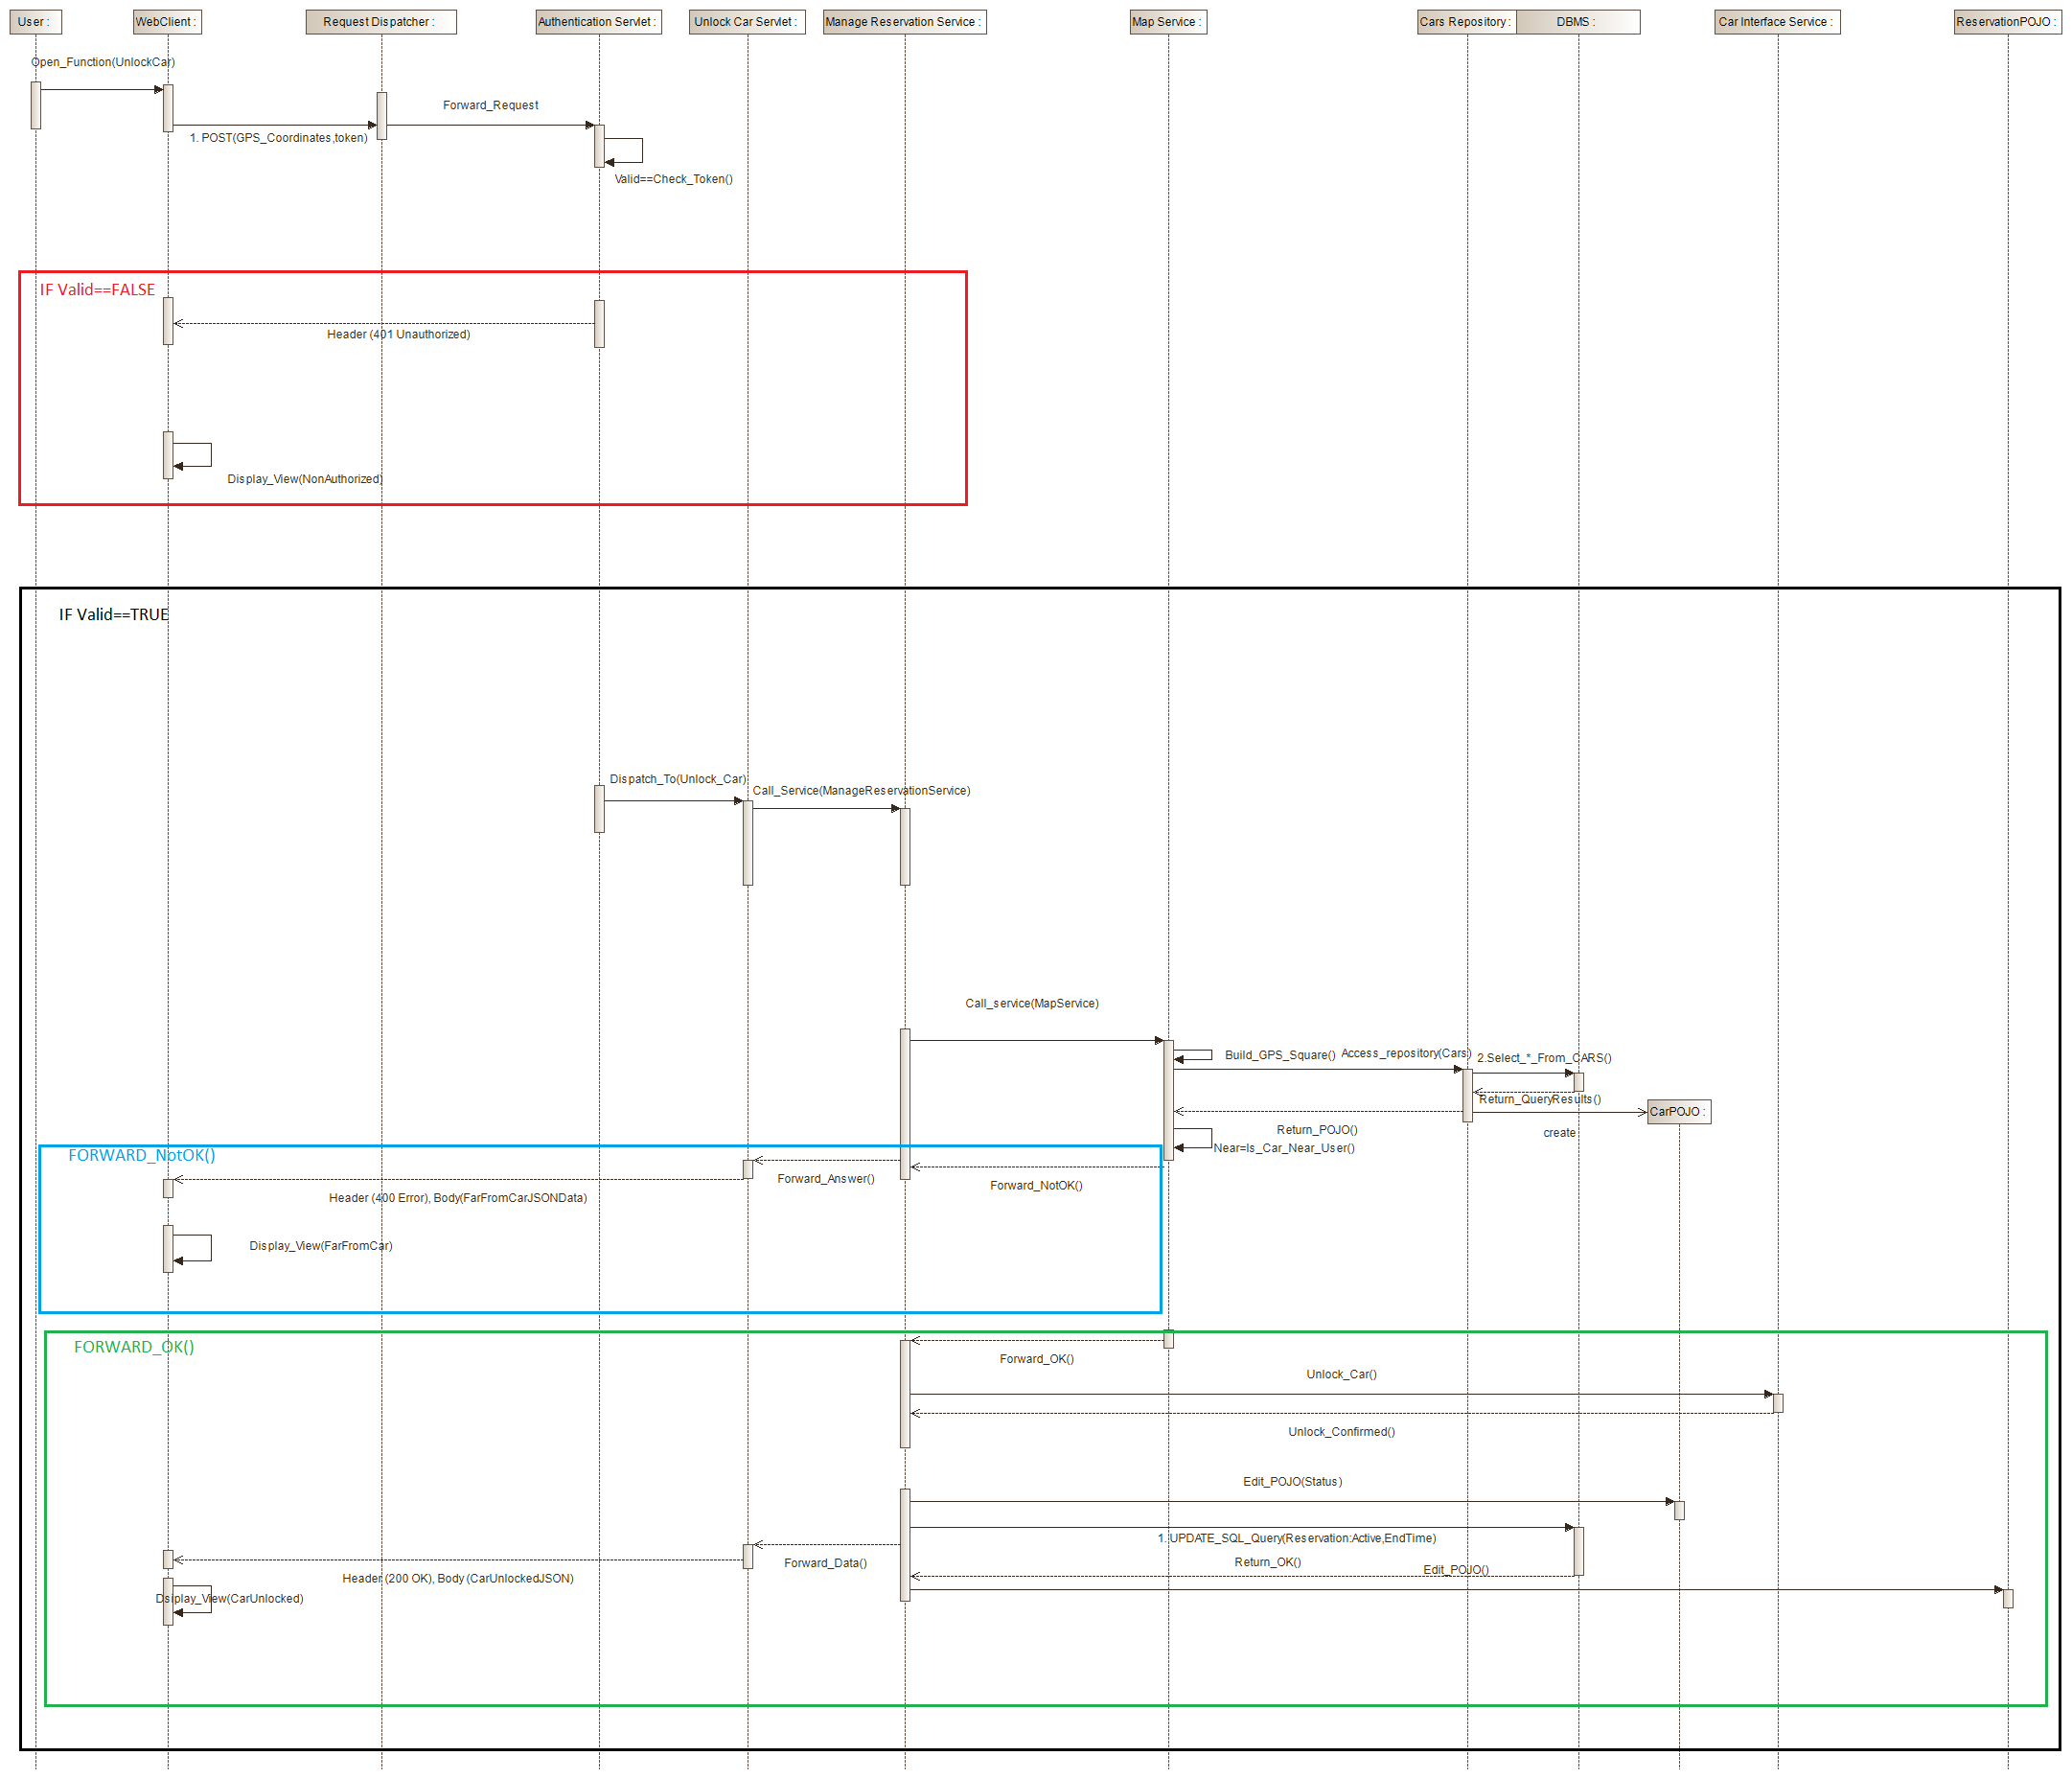
\includegraphics[width=\textwidth]{../Images/Sequence_Final/Unlock_Car}
	\caption{Unlock Car}
\end{figure}
The User can perform this action only via MobileAPP, after performing ReserveCar.
\begin{enumerate}
	\item[1.] PUT(“/unlock/{reservationid}”,body(“reservation=…token=..”))
	\item[2.] We perform a SQL query to check if the User is nearby the car. We previously built a GPS User’s coordinates square so we check if the car GPS coordinates are inside this square to unlock the Car.
\end{enumerate}
\clearpage
\subsubsection{Drive Car}
\begin{figure}[h]
	\centering
	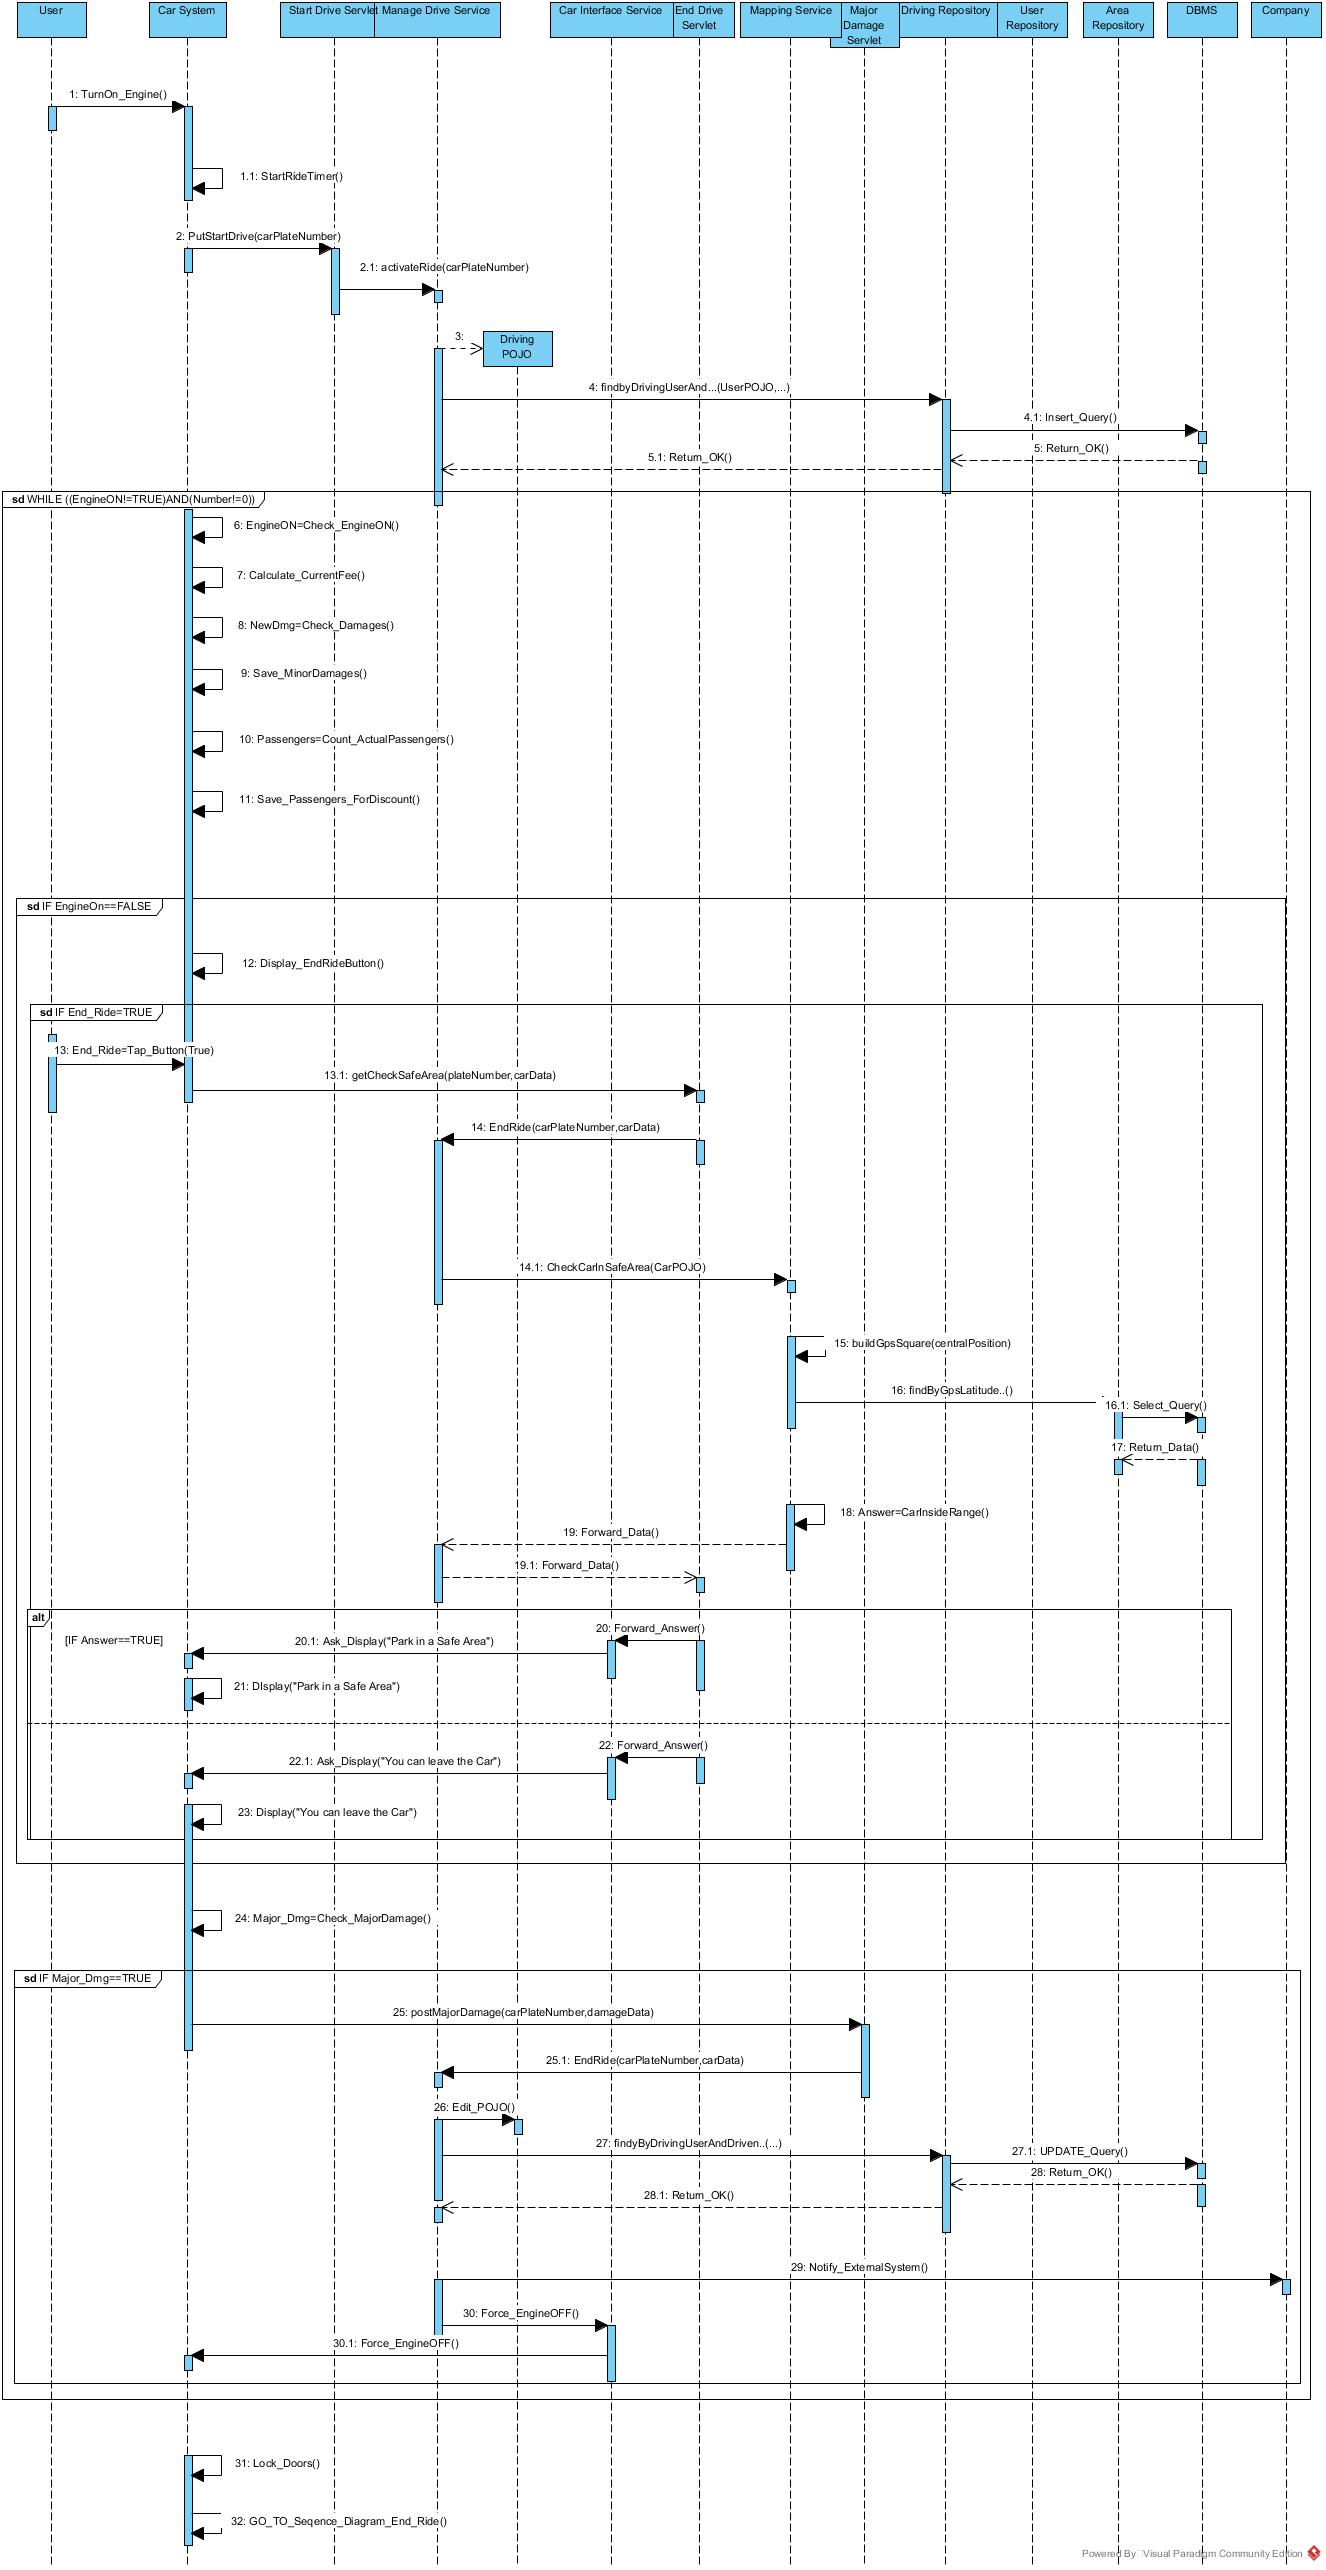
\includegraphics[width=\textwidth]{../Images/Sequence_Final/Drive_Car}
	\caption{Drive Car}
\end{figure}
For this Action the MobileApp is not required.
We take as an assumption that when a Major Damage happens the people will leave the car.
\begin{enumerate}
	\item[1.] We perform a SQL query to check if the Car is inside a SafeArea. We previously built a GPS Car’s coordinates square so we check if the Area GPS coordinates are inside this square and so if the Car is regularly parked.
	\item[2.] We perform a SQL query to check if the Car is inside a SafeArea. We previously built a GPS Car’s coordinates square so we check if the Area GPS coordinates are inside this square and so if the Car is regularly parked.
\end{enumerate}
\clearpage
\subsubsection{End Ride}
\begin{figure}[h]
	\centering
	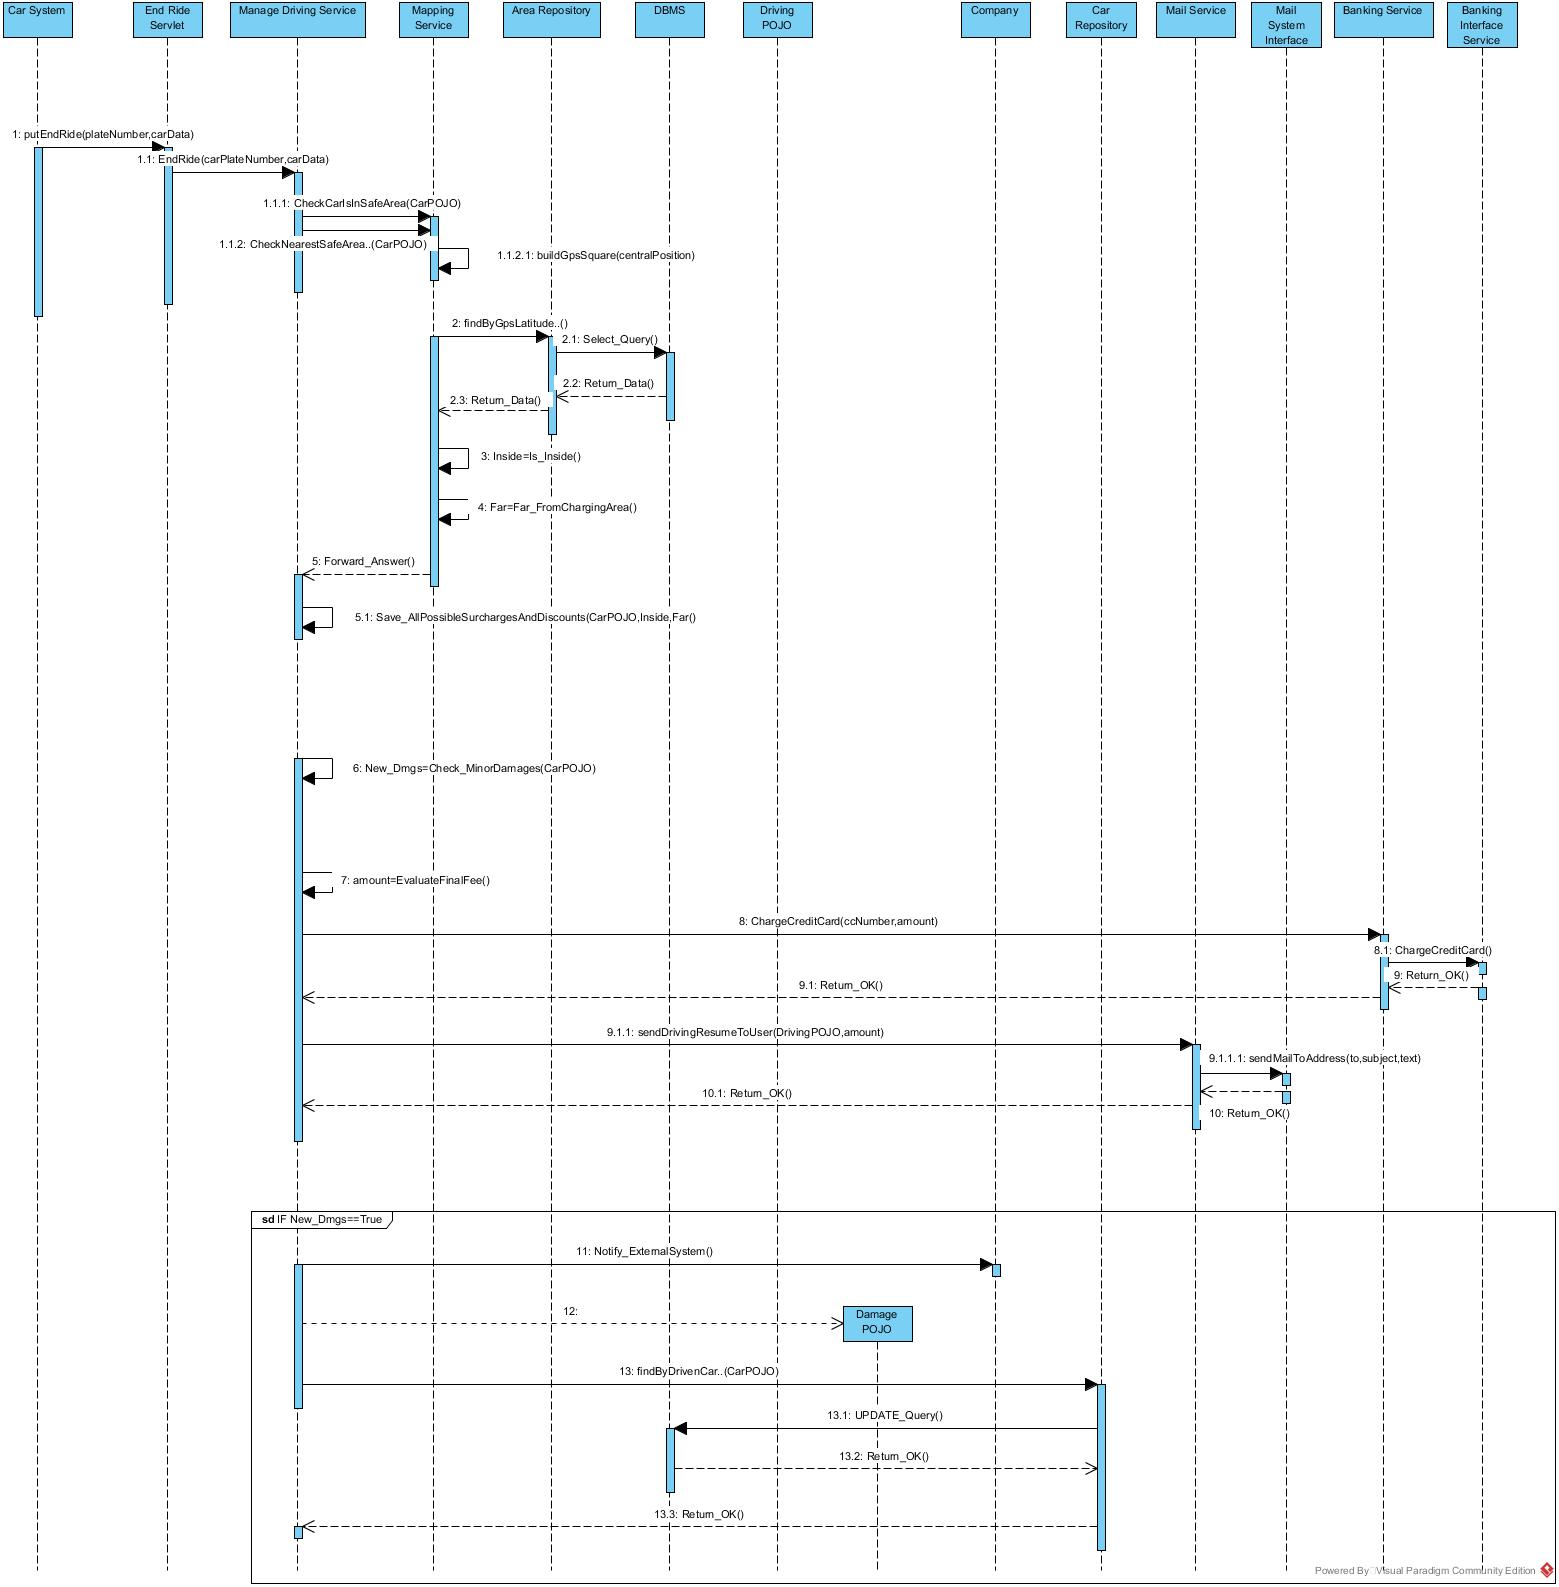
\includegraphics[width=\textwidth]{../Images/Sequence_Final/End_Ride}
	\caption{End Ride}
\end{figure}
For this Action the MobileApp is not required.
\begin{enumerate}
	\item[1.] We perform a SQL query to check if the Car is too far from a ChargingArea. We previously built a GPS Car’s coordinates square so we check if the Area GPS coordinates are outside this square and so if should apply a surcharge to the User’s fee.
	\item[2.] We perform a SQL query to store the Car damage in the Car Table of the Database.
\end{enumerate}
\clearpage
\subsubsection{Money Saving Option}
\begin{figure}[h]
	\centering
	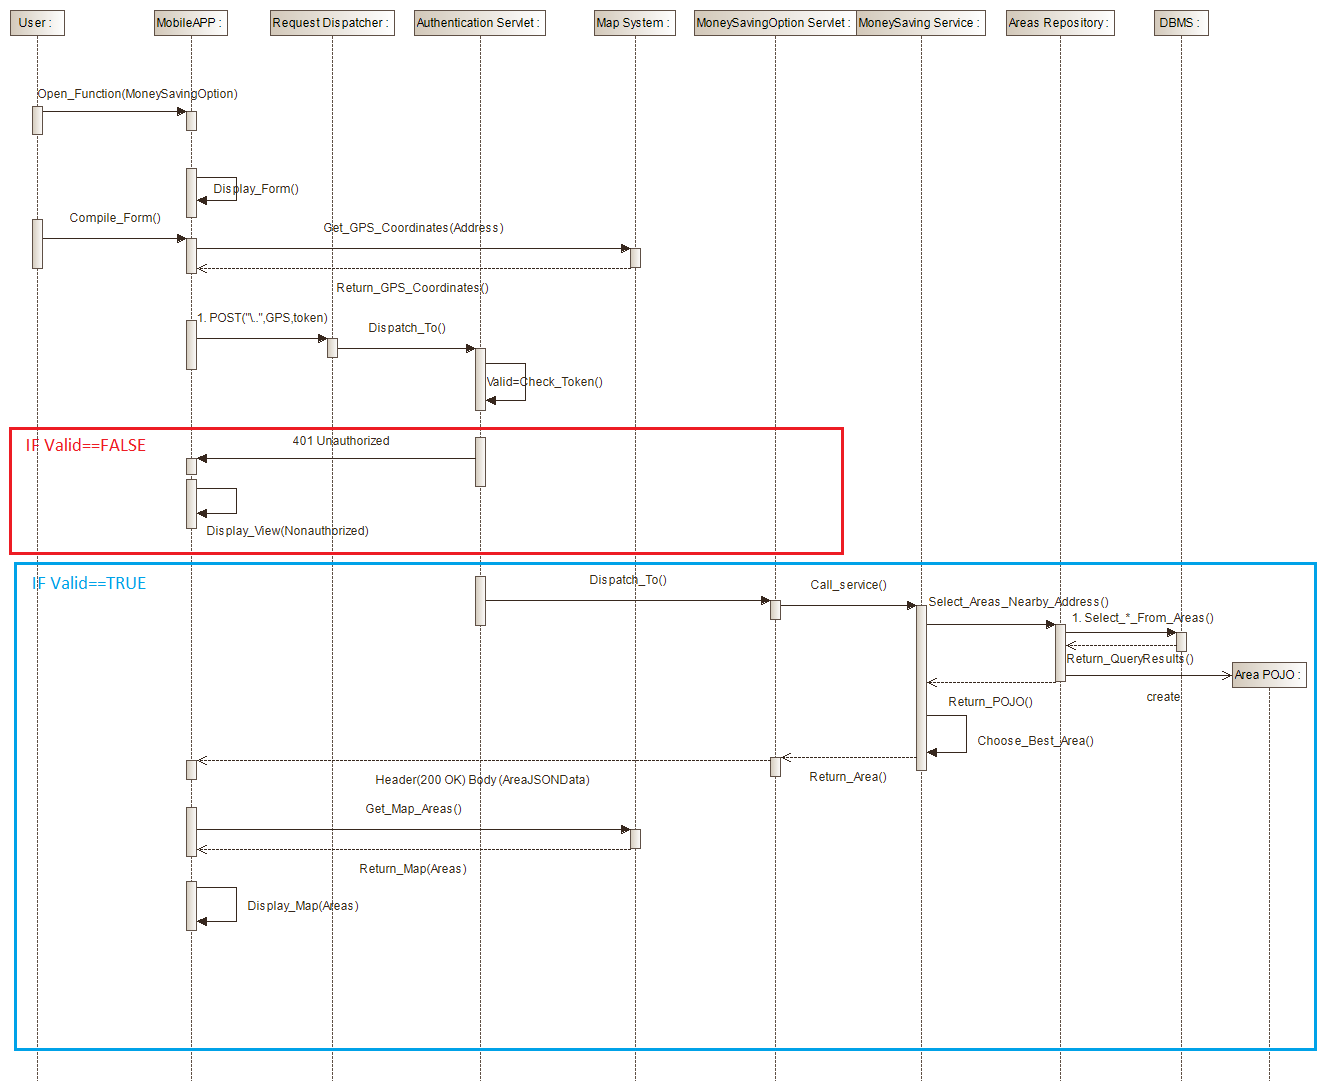
\includegraphics[width=\textwidth]{../Images/Sequence_Final/Money_Saving}
	\caption{Money Saving Option}
\end{figure}
The User can perform this action via MobileAPP only.
We take as an assumption that there's a background task in the system which constantly retrieve data from the Areas.
\begin{enumerate}
	\item[1.] We perform a SQL query to return the Areas which are inside a determined size square from the User’s desired address.
\end{enumerate}
\clearpage


\subsection{Component Interfaces}
The System is based on the Spring framework (see \ref{Spring}) and uses its interfaces. For the rest, the Class Diagrams should provide all the necessary information.

\subsection{Protocols}
The Model, View and Controller macrocomponents communicate with each other through a number of protocols:
\subsubsection{HTTP}
HTTP, HyperText Transfer Protocol, is the hypermediaexchange protocol that is the basis of the World Wide Web. An analysis of the HTTP protocol is beyond the scope of this document, however it has to be mentioned, since Registration can be performed via the Company website, which is HTTP-based. Therefore, communication between the Web Client (the website itself, accessed through the User or Visitor's browser) and the Server will be managed through HTTP requests and dynamic JSP pages.

\subsubsection{API queries}
Parts of our System rely on external services: the Maps component, for instance, will send requests to an external API to obtain maps for the desired location, and in the same way the Banking component will process payment by sending requests to an external banking system's API. All communication between the APIs and the Controller will make use of the HTTP protocol.

\subsection{Architectural Style}
The System will be mainly built according to three different architectural patterns: Model-View-Controller (MVC for short), Client-Server multitier and REST. 
Furthermore, the Application will be mainly built using the Spring framework. Further details can be found in section \ref{Spring}, which can easily cope with the architectural decision previously mentioned.

\subsubsection{MVC}\label{MVC}
The Model-View-Controller design pattern is a tried and tested paradigm that has proved itself to be effective and efficient. By separating the application in three macrocomponents, it allows for full encapsulation, with all the related advantages: each component can be changed without hassle, since they only need to present a coherent interface to the other ones, and it is easy to perform integration testing even if one or more components haven't been fully implemented.

The User Application will make up the View macrocomponent. It will display data from the Model and tell the Controller the actions to perform. It would interface with the rest of the system through a Java servlet, allowing information to be transferred seamlessly over a networked connection.

The Server-Side Application will make up the Controller macrocomponent. According to the requests of the View, the various parts of the Controller will read and, in some cases, modify the data stored in the Model, then send the appropriate data back to the View, allowing the User to make further decisions. The Controller would be divided into several components, each one interfacing with a different component of the Model: a Database Controller, for instance, would access the Database to retrieve information about the Users and the Cars, while the Maps Controller would get data from the Maps API.

The Model macrocomponent would be made up of many different components, each representing a different subset of the data required by the application: the Controller would have access to the data stored, to display them via the View. Different data subsets would be handled differently: the Database, for example, will allow the Controller to change the data, but external APIs will only provide the required information.

For web applications such as the ones we are developing, the MVC paradigm comes naturally, since these applications are naturally divided in three main components: a GUI running from the user's smartphone and the Web Browsers are the View macrocomponent, the Server-side code is the Controller, while the SQL database is the Model.

\subsubsection{Multi-tier Server-Client}
We mentioned above that we are using a client mobile application the user will interact with, while a large server will perform most of the computation. This is called \emph{Server-Client approach}, and it is used in most web application.

There are several reasons to choose this approach over having every instance of the application fulfill the duties of both the View and Controller macrocomponents: first and foremost, the client application can be kept lightweight, allowing it to be used even on low-end smartphones. Since the client needs to perform close to no computation, only handling communications, the application can easily run on most platforms.

Another advantage is that if every client application processed its requests at the same time, there would be a significant chance of collision: for example, two users could reserve the same car at the same time. With a server-side application, collisions can be readily detected and resolved.

Finally, having a centralized server application allows for much quicker communication with the database, which is necessarily centralized.

Other than for the mobile application, the Server-Client approach will be used to manage communication between the server and the Cars: every Car will be outfitted with a small computation unit tasked with collating sensor data. It will be this Car system that will calculate, update and show the current Fee, detect damage, check for the presence of Passengers and communicate with the Server when the Ride ends, either because the User wants to or because the Car has sustained major damage.

To enable the system to cope with flexibility and reusability, we have also segregated our System into tiers, a practice that ensure that we can decide at a later point to modify or add a specific layer, instead of reworking the entire System.
So, the application will be divided into several layers:
\begin{enumerate}
	\item Database
	\item Entities (Persistence Layer)
	\item Repositories (Data Access Layer)
	\item Services (Business Logic Layer)
	\item Controllers (Communication Layer)
	\item Thin Client
\end{enumerate}
All layers except the last one make up the Server Tier.

\subsubsection{RESTful web service}\label{sec:rest}
The communication between the thin client making up the View and the server-side Controller application is set up according to the REpresentational State Transfer set of constraints. Data exchange is also made through the HTTP protocol, using SSL to provide encryption of sensible data, but the data are codified in the JSON format, according to the REST constraints.

Complying with the REST constraints allowed not only for simple component design, but also for intermediate layers such as firewalls or proxies. That is because the stateless nature of the system means that every request sent by the client contains all the necessary information for processing, not relying on server-side information. Furthermore, using a RESTful service allows us to design a uniform interface, easily allowing for future scalability.

The communication between the Cars and the Servers will be REST-compliant as well.

\subsection{Other design decision}
\subsubsection{The Spring Framework} \label{Spring}
Spring is an open-source, modular application framework generally used to build web applications on top of the Java EE platform. It provides a plethora of functionalities, from high-level servlet control to security services, that can be used by Java-based web applications. One core feature of Spring is that it can be used on any deployment platform: therefore the development team can focus on building the application without being constrained by the target platform's specifications, and the application could be easily deployed to a different target with minimal effort.

Spring is focused on the Inversion of Control pattern, according to which the programmer should not create objects, rather specify how objects should be created, then delegate that responsibility to an external object or service. This is extremely useful because, according to the Java Persistence Standard, objects will need to be dynamically created at runtime.

Spring allows to use annotations to classify the servlets that we are creating into several stereotypes: here are the ones that we are using.
\begin{description}[leftmargin=!,labelwidth=\widthof{\bfseries @Repository}]
	\item[@Repository] Repositories control access to databases, retrieving the information needed to create Entities. Repositories manage database and API queries, providing a Data Access Layer to control information and exchange it with the Persistence Layer.
	\item[@Controller] Controllers are used for connecting the client to the server, managing HTTP requests, and invoking Services. Their function is to translate HTTP requests to functions and viceversa, providing an interface for client-server communication. For the Car and Mobile clients, which have more responsibilities than the simple Web Client, a specialization \textbf{@RESTController} will be used, allowing us to provide a simple RESTful interface.
	\item[@Service] Services make up the Business Logic Layer. We provide two specializations of Service, \textbf{@InternalService} and \textbf{@ExternalService}: the former will handle internal logic, such as gathering relevant information to send to the Client, performing checks on Cars and Users, or calculating the optimal Charging Areas for users using the Money Saving Option, while the latter will provide an interface for the external services such as Mapping or Banking. Services will interact with Controllers for client-server communication and with Repositories for data access and modification.
\end{description}

\subsubsection{Server Specifications}
\label{server}
\paragraph{Tomcat}\label{par:tomcat}
While Spring provides tool for working with servlets, they would be implemented through the Apache Tomcat container and HTTP server. An open source project, Tomcat has been extensively tested and is known for its stability, performance and scalability, also providing excellent documentation and community support. Furthermore, there is an edition focused for Java EE, called TomEE, which integrates flawlessly with Spring.

\paragraph{NGINX}\label{par:nginx}
In order to manage requests, allowing the server to be easily contacted by the clients is paramount. In order to do that, an easy way is introducing an intermediary called a reverse proxy, tasked with retrieving resources according to incoming requests, reducing the risk of overloading the server.

NGINX is an open source reverse proxy that can also act as an HTTP server. It can be set to integrate flawlessly with Tomcat and enables the server to manage thousands of simultaneous connections without any drop in performance. Again, NGINX has an extensive documentation and community support.

\paragraph{Forward Proxy and Firewall}
In order to contact External Services, the System sends requests through a forward proxy. This ensures that the System will present a unified outbound interface for HTTP requests. We chose to use tinyproxy for that, because it's lightweight and compatible with Tomcat.

We also assume that the database will be protected by a Firewall. It is worth noting that, for this reason, the Application servers should be on the list of trusted addresses.

\subsubsection{Scenarios}
During the writing of this document, a case has been repeatedly brought forward and analyzed: that is, what happens when a User wants to leave the car for a relatively short amount of time and not have someone reserve it, possibly leaving them without a ride?

Several solutions have been considered. In the end, our solution was to introduce a "End Ride" button on the screen of the Car system. This way, even if the User kills the engine and exits the Car, the doors are not locked and the Ride does not end unless that button is pressed. As a side-effect, this makes it less likely for the user to forget their belongings, in the Car, since it would not lock unless the User had pushed the button.

Of course, there is an undesired side-effect as well: since the Car is unlocked, it would be possible for a malicious passerby to get in the Car and drive away. Since Cars can be remotely operated, a User could notice it readily and notify the Company to ask for intervention, but it is recommended that the Terms and Conditions specify that the User may be held liable for any such misdemeanor. A User who is worried about this happening should end the ride before leaving the Car, then immediately Reserve it again through the Mobile application.

Furthermore, in order to minimize the chance of someone forgetting to press the "End Ride" button, the Mobile application will receive regular notifications whenever the associated Car is empty but still In Use.

\clearpage
\section{Algorithm Design}
In this section, the two most complex algorithms in the System will be explained.
\subsection{Build Square}
This is the algorithm that, given a start position, returns a set of GPS coordinate bouns that form a dX * dY rectangle centered on that position
The bounds are calculated via the formula\\
\verb&new_latitude = latitude&$\pm$\verb&(dy*k)&\\
\verb&new_longitude = longitude&$\pm$\verb&(dx*k)/cos(latitude*pi/180)&

The constant $k$ is equal to $\frac{180}{\pi\cdot r}$, where $r$ is the radius of the Earth, approximately 6378 kilometers. The $dx$ and $dy$ values are the offset in longitude and latitude. It should be noted that this conversion is only accurate if these values are small compared to $r$.

This algorithm is used several times in the project. One example is when the System locates the available Cars near the User, another is when it checks whether the User is close enough to the Car to unlock it.

\subsection{Money Saving Option}
In order to find the optimal Charging Area where to park the car, the System will need some kind of metrics to evaluate the possible choices. Therefore, this algorithm will assign a score to each Charging Area within reasonable distance of the user (default 1 km) and return the address of the one with the highest score. The \verb+calculateBounds()+ function is shown in the above subsection.

The weights $W_l$, $W_m$ and $W_n$ are defined, defaulting to values of 100, 5 and 10 respectively.

\begin{algorithm}[H]
 \KwData{a starting position destPos}
 \KwResult{the address of a Charging Area}
 bounds = calculateBounds(destPos)\\ 
 areas = SQLQuery(Charging Areas within the bounds)\\ 
 set maxScore to minus infinity\\ 
 set bestArea to NONE\\ 
 \ForEach{a in areas}{
  set score to 10\\  
  score = score - distance(destPos, a.position())/$W_l$\\ 
  score = score + (a.freeSockets/a.totalSockets)$\cdot W_m$\\
  score = score - (a.parkedCars/a.totalSpots)$\cdot W_n$\\  
  \If{freeSockets == 0}{
   set score to minus infinity
   }
  \If{score $>$ maxScore}{
   set bestArea to a
   }
  }
 \textbf{return} bestArea.address

\end{algorithm}
%TODO Simone: dobbiamo aggiungere l'algoritmo per il calcolo della finale fee (i vari casi di surcharge e disount)
\subsection{Calculate Final Fee}
This algorithm is used to calculate the final Fee that a User will have to pay, comprehensive of surcharges and discounts.

\begin{algorithm}[H]
 \KwData{a DrivingPOJO object containing details about a Ride}
 \KwResult{the final Fee}
 startFee = (Ride.timeEnd - Ride.timeStart)*feePerMinute\\
 feeMultiplier = 1\
 \If{Ride.hasPassengerDiscount}{
  feeMultiplier = 0.9
 }
 \If{Ride.hasHighBatteryDiscount}{
  feeMultiplier = 0.8
 }
 \If{Ride.hasPluggedCarDiscount}{
  feeMultiplier = 0.7
 }
 \If{Ride.hasAwayFromChargingAreaSurcharge {\bf or} Ride.hasLowBatterySurcharge}{
  feeMultiplier = feeMultiplier + 0.3
 }
 \textbf{return} startFee*feeMultiplier

\end{algorithm}

\clearpage
\section{User Interface}
\subsection{Mockups}

\begin{figure}[h!]
    \centering
    \begin{subfigure}[b]{0.45\textwidth}
        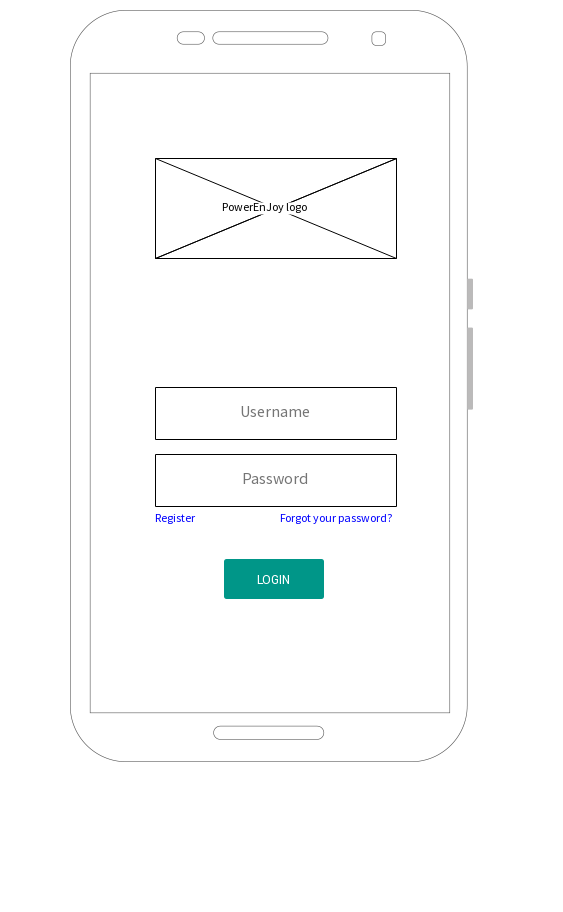
\includegraphics[width=\textwidth]{../UI/LoginScreen}
        \caption{Login Screen}
    \end{subfigure}
    ~
    \begin{subfigure}[b]{0.45\textwidth}
        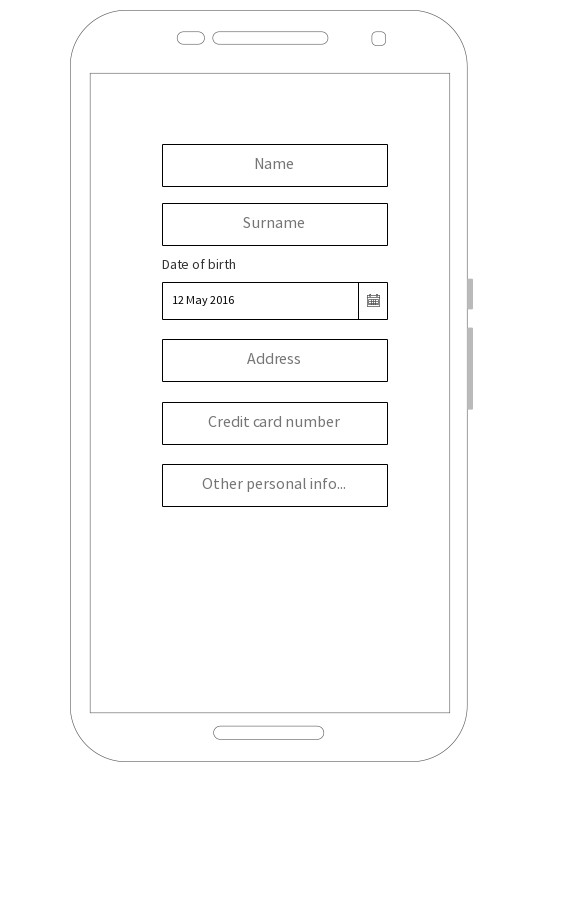
\includegraphics[width=\textwidth]{../UI/RegisterScreen}
        \caption{Register Screen}
    \end{subfigure}
\end{figure}
The Login and Register Screens are the only parts of the application that are accessible to Visitors. Registration can also be performed through the Company website, or Web Client. A User who logs in can access the Main Screen.\clearpage

\begin{figure}[h!]
    \centering
    \begin{subfigure}[b]{0.45\textwidth}
        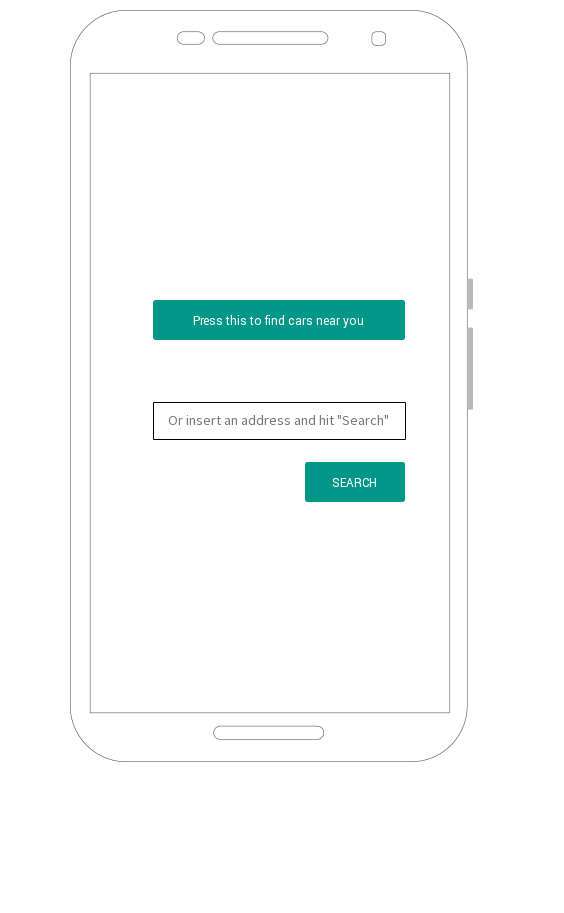
\includegraphics[width=\textwidth]{../UI/MainScreen}
        \caption{Main Screen}
    \end{subfigure}
    ~
    \begin{subfigure}[b]{0.45\textwidth}
        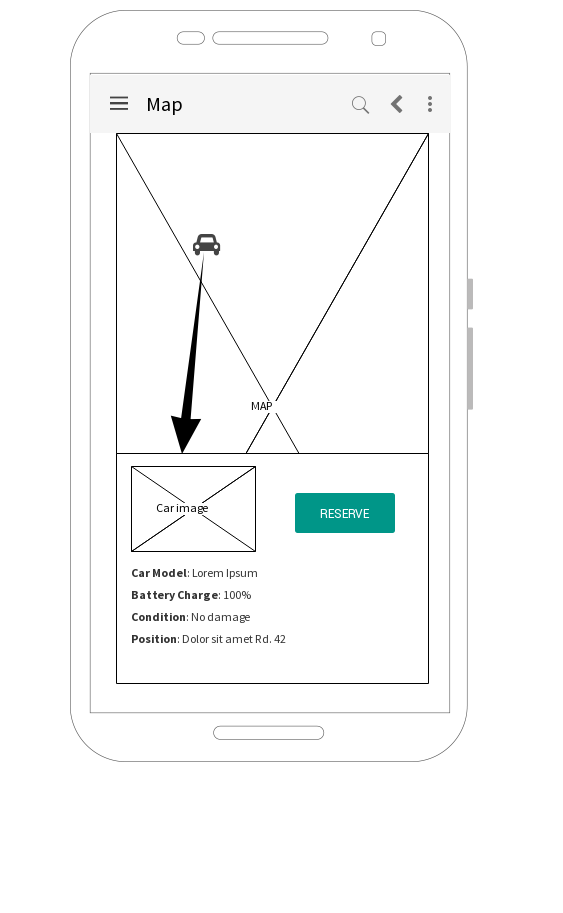
\includegraphics[width=\textwidth]{../UI/MapScreen}
        \caption{Map Screen}
    \end{subfigure}
\end{figure}
The Main Screen allows the User to view Cars near either their position or an address of their choice. From the Main Screen, the application shifts to the Map Screen, where all the eligible Cars are shown on a map, together with the position of the User. From this screen, the User can select one of the Cars shown and reserve it.\clearpage

\begin{figure}[h!]
    \centering
    \hspace{-2cm}
    \begin{subfigure}[b]{0.45\textwidth}
        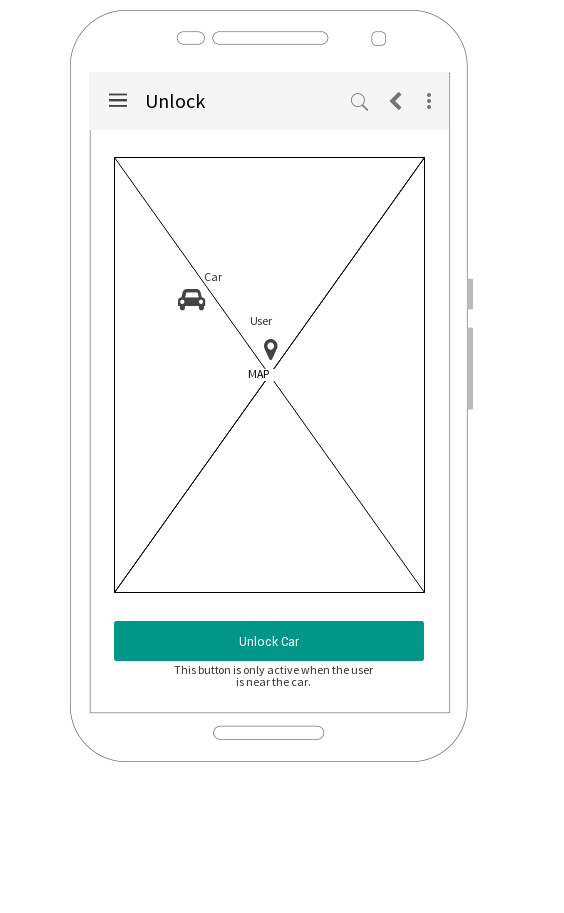
\includegraphics[width=\textwidth]{../UI/UnlockScreen}
        \caption{Unlock Screen}
    \end{subfigure}
    ~
    \begin{subfigure}[b]{0.64\textwidth}
        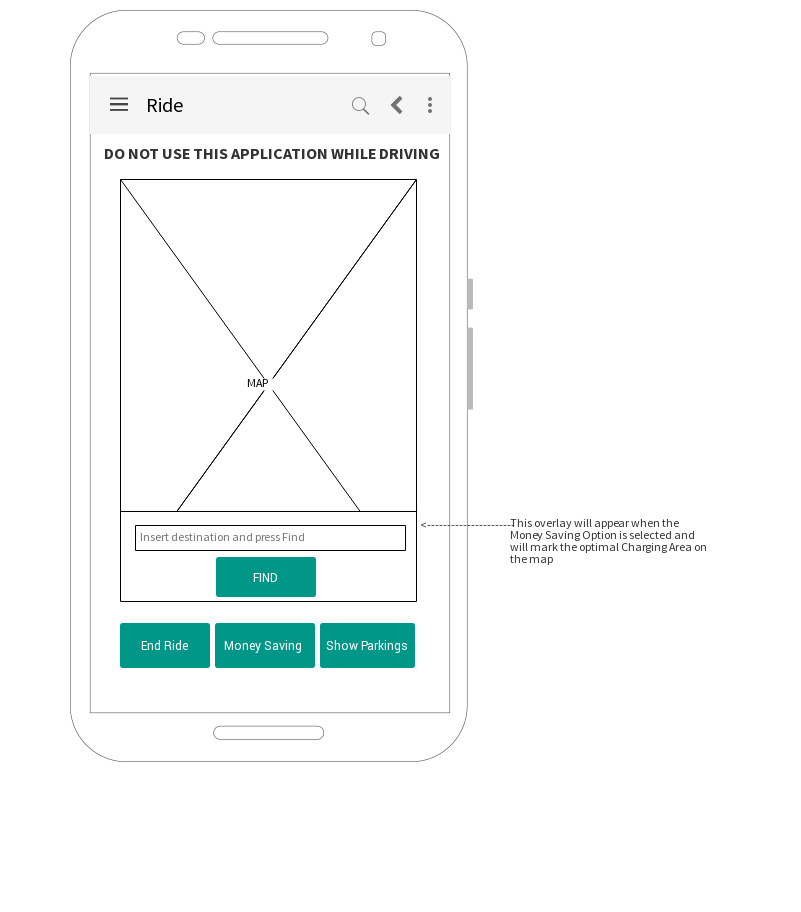
\includegraphics[width=\textwidth]{../UI/RideScreen}
        \caption{Ride Screen}
    \end{subfigure}
\end{figure}
After reserving a Car, the application will pass to the Unlock Screen, containing a map showing the User's position and that of the reserved Car. When the system detects that the User is close enough to the Car, the Unlock Car button becomes available.

While the Car is In Use, the application shifts to the Ride Screen, showing a map with the position of the User and allowing them to show on it the available Parking Areas or select the Money Saving Option to be notified of the optimal Charging Area where to park the Car. \clearpage

\begin{figure}[h!]
	\centering
	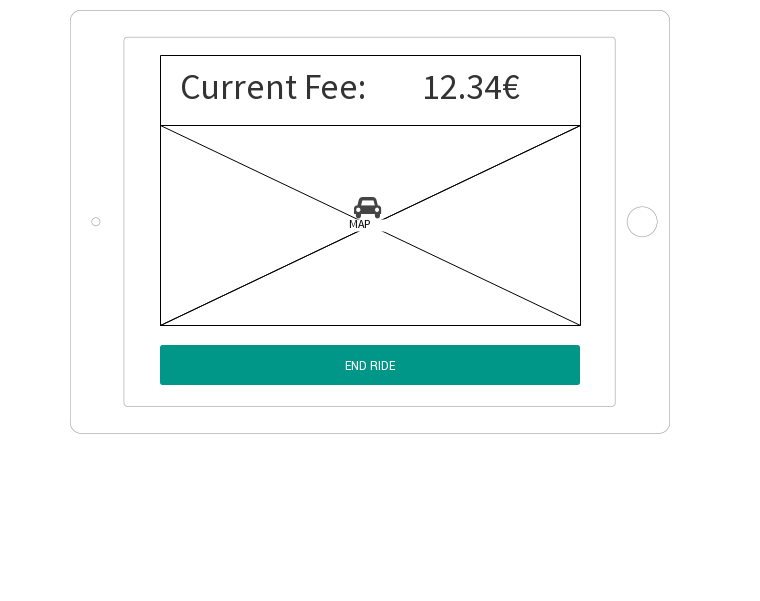
\includegraphics[width=0.9\textwidth]{../UI/CarScreen}
	\caption{Car Screen}
\end{figure}

The Car will have an internal computer showing a map of the area, the current Fee (not including any discount the User might be eligible for) and an "End Ride" button. Not pressing the button when leaving the Car will leave it In Use so that the User may leave the Car for a while if necessary (e.g. going to buy things without worrying that someone other might reserve the Car). However, it is worth noting that the Car is kept unlocked, and the User should be legally responsible for any improper use, theft or damage to the Car.

When the End Ride button is pressed, the Car will check to be parked in a Parking Area, then communicate all relevant data to the server.

\clearpage
\section{Requirements Traceability}
\begin{enumerate}
	\item[G1] The System should allow the registration of the Visitors with their credentials and payment informations.
	\item[-] The Client allows to do that through the Register Screen of the Mobile Client or through the Web Client.
	\item[G2] The System should allow all Users to use all the functionalities reserved to them.
	\item[-] All User functionalities are accessible through the Mobile Client.
	\item[G3] The System should be able to give each User the list of all the available cars in a range of 5KM from his/her GPS position or a specific address.
	\item[-] The Locate Cars Controller does that.
	\item[G4] The System should allow each of its Users to reserve a Car whose state is Available.
	\item[-] The Reserve Car Controller does that.
	\item[G5] If an User has reserved a Car and he/she did not unlock it within 1 hour from the reservation, the System sets the Car state as Available, the reservation expires and the user pays a fixed Fee of 1 EUR.
	\item[-] Included in the responsibilities of the Reserve Area Controller.
	\item[G6] The system should allow each User to unlock a previously reserved Car when he/she is in a distance range of 15 meters from the same Car.
	\item[-] The Unlock Car Controller does that.
	\item[G7] The system should allow each User to drive a Car which he/she has previously unlocked.
	\item[-] Once Unlocked, a Car can be driven.
	\item[G8] The System should be able to know the time usage of the Car, misured in minutes.
	\item[-] The DrivingPOJO stores that information.
	\item[G9] The System should allow Users to know where are the Parking Areas.
	\item[-] The Locate Areas Controller does that.
	\item[G10] The system should allow each User to end the ride in a Parking Area.
	\item[-] The End Ride action is available on a parking area.
	\item[G11] If the System detects the User took at least two other passengers onto the Car, the system applies a discount of 10\% on the last ride.
	\item[-] The Final Fee algorithm considers that.
	\item[G12] If a Car is left with no more than 50\% of the battery empty, the System applies a discount of 20\% on the last ride.
	\item[-] The Final Fee algorithm considers that.
	\item[G13] If a Car is left at special parking areas where they can be recharged and the User takes care of plugging the Car into the power grid, the System applies a discount of 30\% on the last ride.
	\item[-] The Final Fee algorithm considers that.
	\item[G14] If a Car is left at more than 3 KM from the nearest Charging Area or with more than 80\% of the battery empty, the system charges 30\% more on the last ride to compensate for the cost required to recharge the car on-site.
	\item[-] The Final Fee algorithm considers that.
	\item[G15] If the User enables the money saving option, he/she can input his/her final destination and the System provides the address of the Charging Area where to leave the Car in order to get a Discount on the total Fee. The Charging Area is determined by the System to ensure a uniform distribution of Cars in the city and depends both on the destination of the User and on the availability of Sockets at the selected Charging Area.
	\item[-] The Money Saving Option controller does that, according to the omonymous algorithm.
\end{enumerate}

\clearpage
\section{Hours of work}
\subsection{Simone Perriello}
\begin{tabular}{l r}
25/11 & 2h\\
30/11 & 2h\\
01/12 & 1h 30\\
02/12 & 3h 30\\
03/12 & 9h\\
04/12 & 4h\\
06/12 & 3h\\
07/12 & 7h\\
08/12 & 7h\\
09/12 & 9h\\
10/12 & 3h\\
11/12 & 8h\\ \hline
01/03 & 5h\\ \hline
TOTAL & 64h\\
\end{tabular}
\subsection{Alessandro Paglialonga}
\begin{tabular}{l r}
30/11 & 2h\\
01/12 & 1h\\
05/12 & 2h\\
06/12 & 4h\\
07/12 & 5h\\
08/12 & 5h 30\\
09/12 & 2h 30 Group Meeting + 4.30 hours Private\\
10/12 & 7h (2h call with Simone)\\
11/12 & 6h (1h call with Simone)\\ \hline
TOTAL & 39h 30
\end{tabular}
\subsection{Enrico Migliorini}
\begin{tabular}{l r}
25/11 & 2h\\
02/12 & 3h\\
03/12 & 3h\\
04/12 & 2h\\
05/12 & 3h\\
06/12 & 2h\\
09/12 & 8h\\
10/12 & 4h 30m\\
11/12 & 8h\\ \hline
TOTAL & 35h 30m
\end{tabular}
\end{document}